\chapter{Identification of Weakly Connected Subsystems (WCSs) for Effective UQ}
\label{chap:wcs}


\section{Proposed Framework for Identification of WCSs}
\label{framework}

In this section, the key features of the proposed framework for the analysis of a stochastic dynamical system and identifying WCSs is discussed. The main idea is to approximate the large dynamical system as multiple weakly connected low-dimension systems~\ref{fig:clusters}. This concept allows us to solve multiple low-dimension problems rather than one large dimension problem. 

\begin{figure}[H]
        \centering
        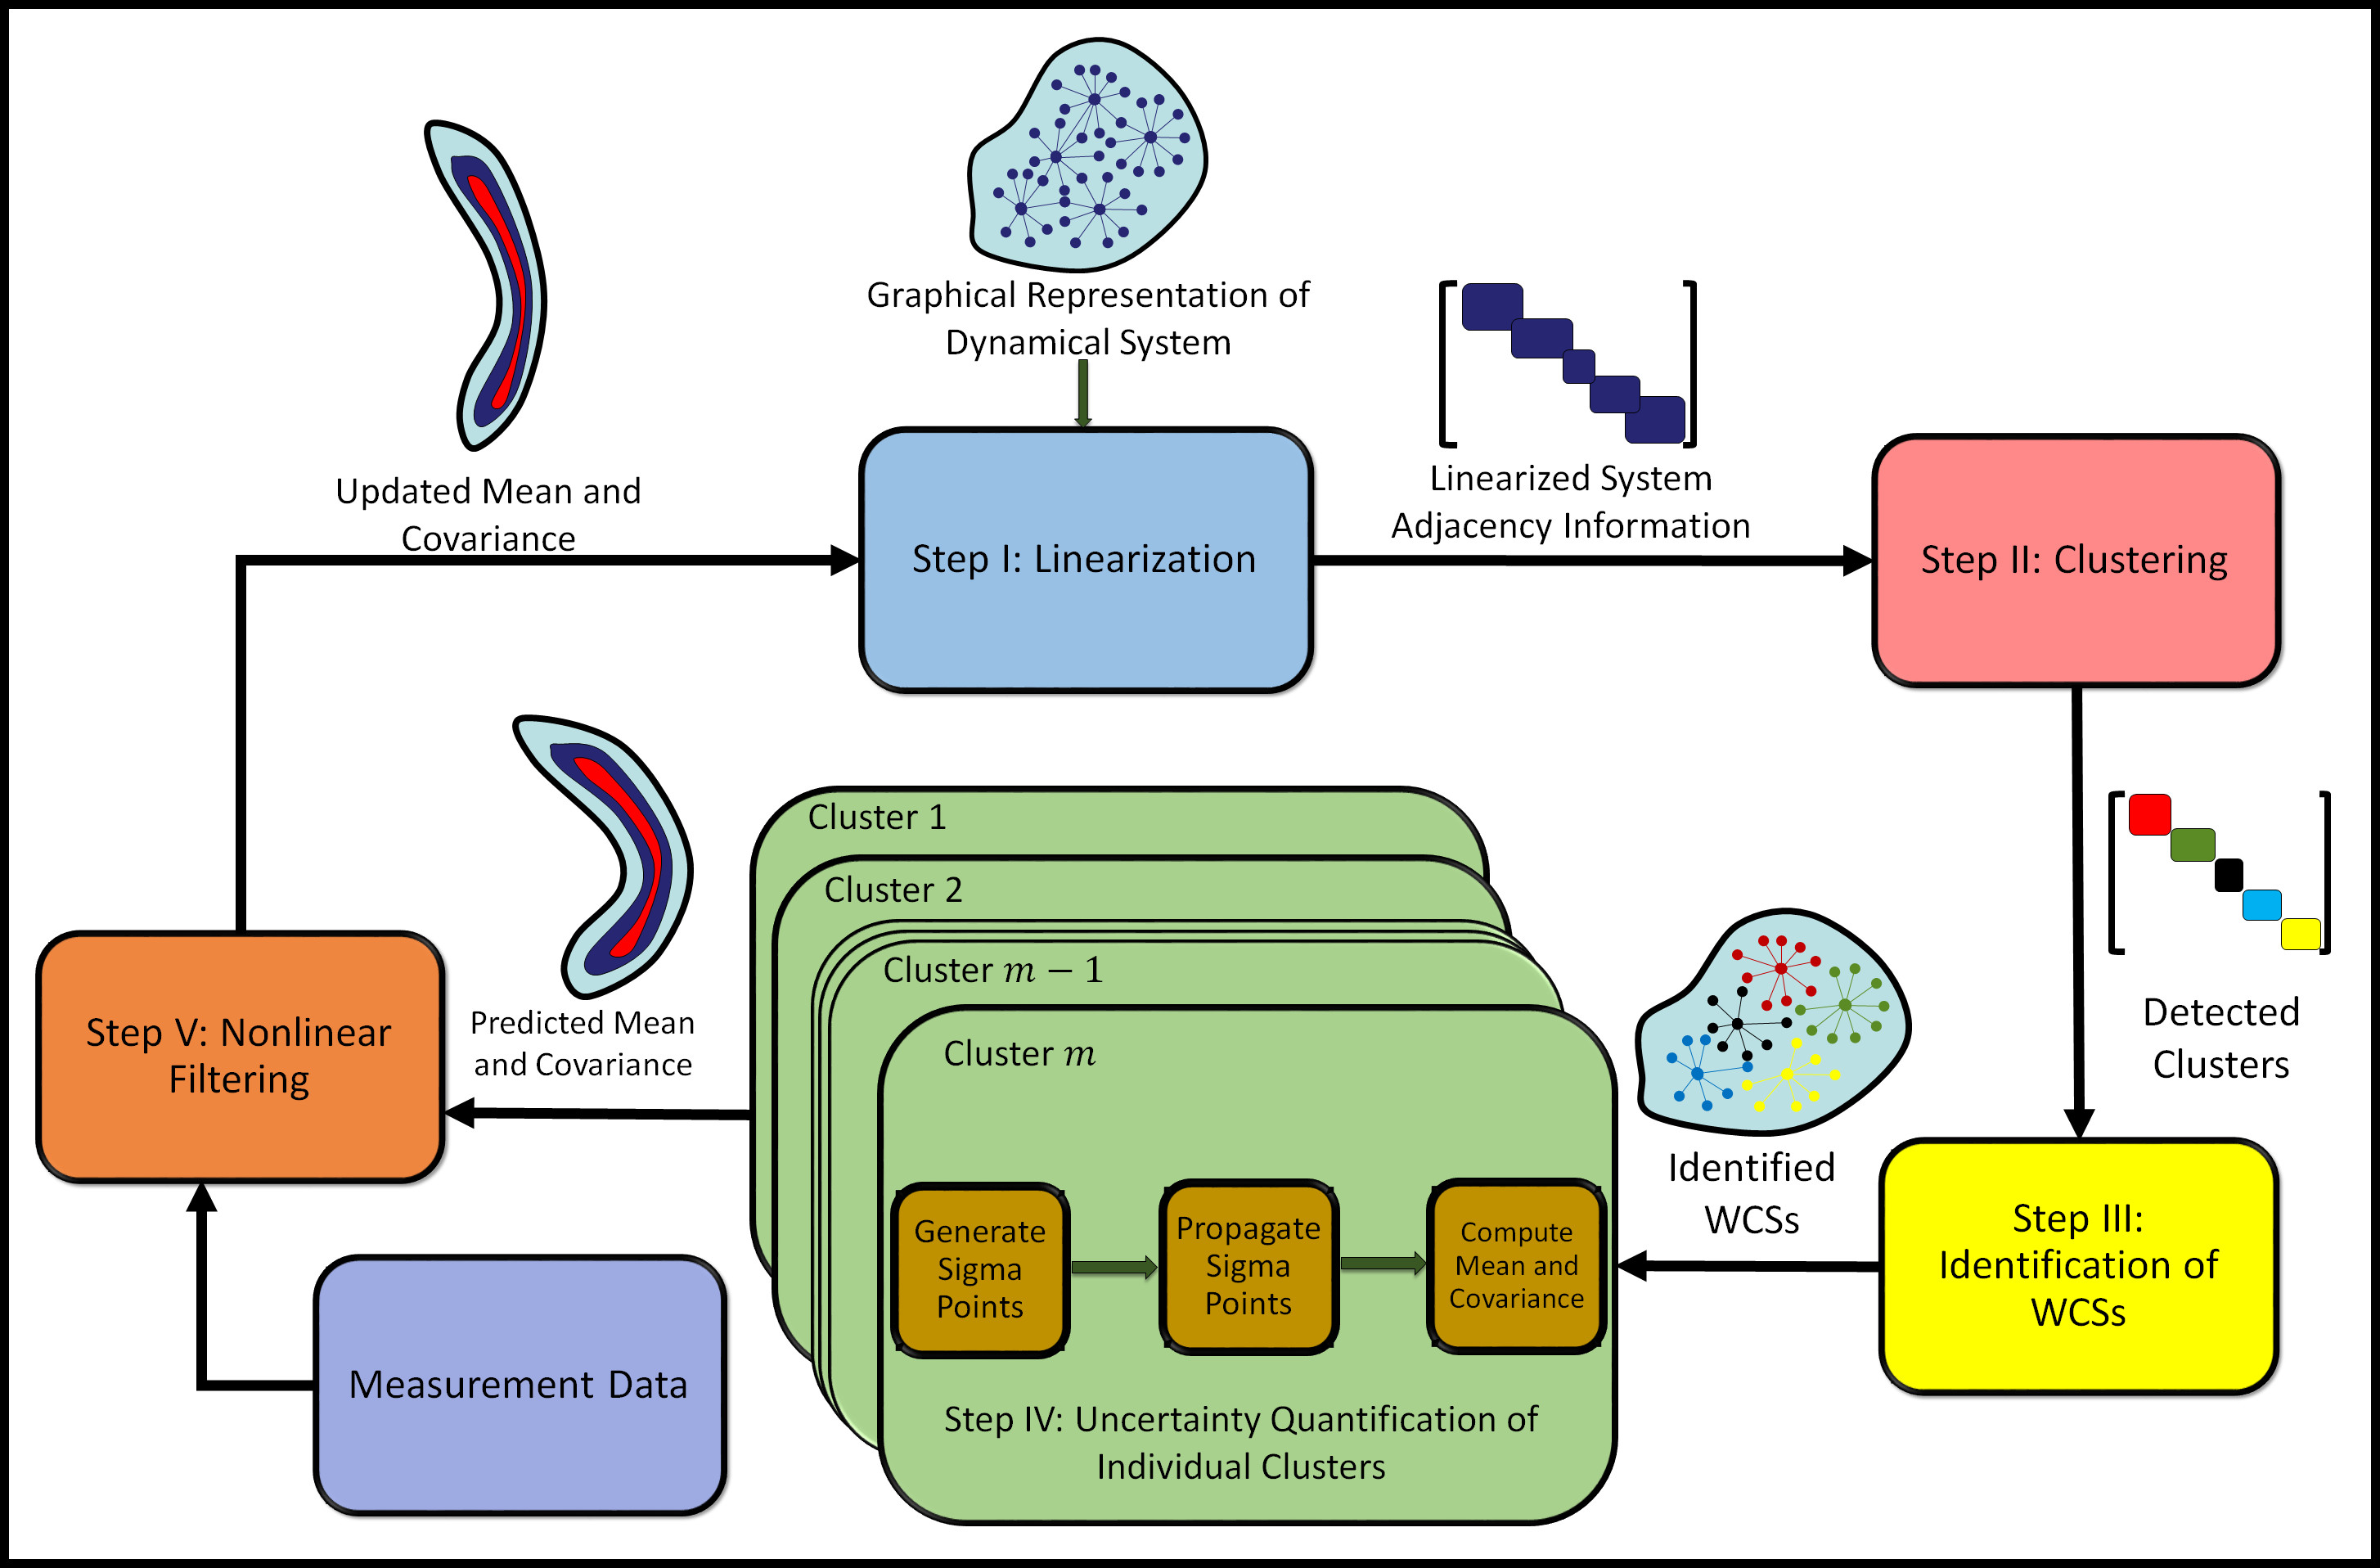
\includegraphics[width=0.8\textwidth]{figures/FIG_2}
        \caption{Determination of Weakly Coupled Subsystems (WCSs): Flowchart explaining the framework for linearization and clustering procedure followed by effective UQ}
        \label{fig:UQframework_2}
\end{figure}

Figure~\ref{fig:UQframework_2} shows the different components of the overall framework. Given a dynamical system with uncertainty in the initial condition, a graph-theoretic representation (as an undirected graph) of the dynamical system is used, where the state variables represent the vertex of the graph. We hypothesize, the graph to be consisting of strongly connected components (or variables) connected by weak edges. These weak edges in conjunction with the clustering methods are used to identify the WCSs. The adjacency or edges in graphical representation are derived from the linear approximation of time derivative of the state vector about the nominal point. In this respect, the first step is to linearize the large dimensional state space in a domain of interest using time and space domain linearization methods. The linearization step helps in quantifying the connectivity information among different state variables (nodes of the graph). The resulting linear system matrix stores the weighted graph adjacency information. Once the graph adjacency matrix is derived from the linearization process, the graph clustering methods are used to identify the clusters in the connected graphs. The next step involves identification of the WCSs. These WCSs are identified by mapping the individual clusters or blocks in the weighted adjacency graph to the state variables involved. The variables of each WCS are used to create the clustered model. The uncertainty quantification methods exploit the identified WCS to propagate the state statistical moments through each WCS, which are updated on the availability of the measurement data. The updated statistical moments are used to define the domain of interest to recompute the adjacency matrix for the clustering methods. Hence, the overall framework is a data-driven cyclic process which goes back to the first step after recalibrating the statistical properties of the state variables on the availability of the data. In subsequent subsections, the details corresponding to the primary steps involved in the proposed framework is outlined.

\section{Weakly Connected Subsystems}

Weakly Connected Subsystems or WCSs are defined as subsystems of the large state space $\mathbf{x}_t \in \mathbb{R}^n$ such that they are approximately decoupled with each other, and their ensemble can approximately replicate the dynamics of the whole system. Mathematically speaking, given the initial value problem defined in Chapter~\ref{chap:uq}, the state space $ \textbf{x}_t \in \mathbb{R}^n$, is clustered into:
\begin{equation}
\label{clustmodel}
\begin{array}{l}
\mathbf{y}_{t_1} = \lbrace x_{t_{11}},x_{t_{12}},\ldots,x_{t_{1n_1}} \rbrace  \\
\mathbf{y}_{t_2} = \lbrace x_{t_{21}},x_{t_{22}},\ldots,x_{t_{2n_1}} \rbrace  \\
\vdots  \\
\mathbf{y}_{t_m} = x_{t_{m1}},x_{t_{m2}},\ldots,x_{t_{mn_1}} \rbrace 
\end{array}
\end{equation}

Where, $\sum_{j=1}^m n_j = n$. Each subset $\mathbf{y}_{t_j} \in \textbf{x}_t$, $j = 1$ to $m$ is termed as a WCS. Each subsystem $\mathbf{y}_{t_j}$ is thus modeled by the ODE defined in $\mathbb{R}^{n_j}$ as 

\begin{equation}
\label{substochdyn}
\dot{\mathbf{y}}_{t_j} = f(\mathbf{y}_{t_j}) \hspace{5 mm} j = 1,2,\ldots,m
\end{equation} 

\noindent The solution is approximated as

\begin{equation}
\label{integral_wcs}
\mathbf{y}_{t_j} =   \mathbf{y}_{t_j} + \int_0^t f(x_{\tau_{j1}},x_{\tau_{j2}},\ldots,x_{\tau_{jn_j}}) d \tau
\end{equation}

\noindent and the moment equation is computed from the reduced order volume integral given as,

\begin{equation}
\label{moment_wcs}
E[\mathcal{G}(\mathbf{y}_{t_j})] = \int  \int \ldots \int_{\Omega_{j \textbf{x}}} \mathcal{G}(x_{t_{j1}},x_{t_{j2}},\ldots,x_{t_{jn_j}}) dP_j
\end{equation}

\noindent where, each random vector $\mathbf{y}_{jt}$, $j = 1,\ldots,m$ is defined on the probability space $(\Omega_{j \textbf{x}},\mathcal{F}_{j \textbf{x}},P_j)$, such that $\Omega_{\textbf{x}}$ is the disjoint union of the countable partitions $\Omega_{j \textbf{x}}$'s. Thus: 
\begin{equation}
\begin{array}{l}
\Omega_{\textbf{x}} =  \displaystyle \bigcup_{j=1}^m \Omega_{j \textbf{x}}  \\
\mathcal{F}_{\textbf{x}} = \mathcal{F}_{1\textbf{x}} \times \mathcal{F}_{2 \textbf{x}} \times \ldots \times \mathcal{F}_{m \textbf{x}} \\
P_{\textbf{x}} = P_1 \times P_2 \times \ldots \times P_m
\end{array}
\end{equation}
Also,
\begin{equation}
P(A_j,A_k) = P(A_j)P(A_k) \text{ for } A_j \in \mathcal{F}_j,A_k \in \mathcal{F}_k, \;\forall \; j \neq k
\end{equation}

Such an approximation can benefit any numerical technique, both deterministic and probabilistic. Instead of solving for the whole system, one can solve for the WCSs $\dot{\mathbf{y}}_{t_j} = f(\mathbf{y}_{t_j})$ in parallel. Now, the theoretical formulation of linearization and clustering that facilitates the identification of WCSs in a high-dimensional nonlinear stochastic system is described in details. 

\section{Approximate Linearization of Nonlinear System}
\label{wcs:linearization}

In this section, mapping schemes are developed to map a nonlinear velocity field to an equivalent linear system matrix. A nonlinear system is defined by a smooth nonlinear velocity field as:
\begin{equation}
\label{nonlindiffeqn}
\dot{\mathbf{x}}_t = f(\mathbf{x}_t )
\end{equation}
where, $f$ does not have the properties of a linear map, and hence a closed form solution is very difficult to obtain. However, one can get some qualitative information of the local behavior of such system.  A good way to get this information of (\ref{nonlindiffeqn}) is to linearize the system about a given point $\mathbf{x}_0$. Expanding $f(\mathbf{x})$ about a point $\mathbf{x}_0$, we get:
\begin{equation}
\label{taylor}
\begin{array}{rl}
f(\mathbf{x}) &= f(\mathbf{x}_0) + Df(\mathbf{x}_0)(\mathbf{x}  - \mathbf{x}_0) + \\ 
&\frac{1}{2} (\mathbf{x}  - \mathbf{x}_0)^T D^2f(\mathbf{x}_0)(\mathbf{x}  - \mathbf{x}_0) + \ldots \\
& = f(\mathbf{x}_0) + Df(\mathbf{x}_0)(\mathbf{x}  - \mathbf{x}_0) + \mathcal{O} ||(\mathbf{x}  - \mathbf{x}_0)^T(\mathbf{x}  - \mathbf{x}_0)||
\end{array}
\end{equation}
The Jacobian $Df(\mathbf{x}_0)$ quantifies the local nonlinearity of a system and gives an approximate linear system. The advantage of such an approximation is that one can formulate ways to solve the system (\ref{nonlindiffeqn}) similar to the linear system defined in Equation~\ref{lindiffeqn}. However, the above formulation linearizes the system about a single point only and hence utilizes only local information. As the system evolves, the Jacobian information of Equation~\ref{nonlindiffeqn} changes over time and the cluster structure changes too. We present two different scheme of linearization, namely \textit{Time-Domain Linearization} and \textit{Space-Domain Linearization}. Figure~\ref{fig_lin} gives a schematic of the two linearization concept using the nominal trajectory and the initial condition uncertainty. 

\begin{figure}[H]
\centering
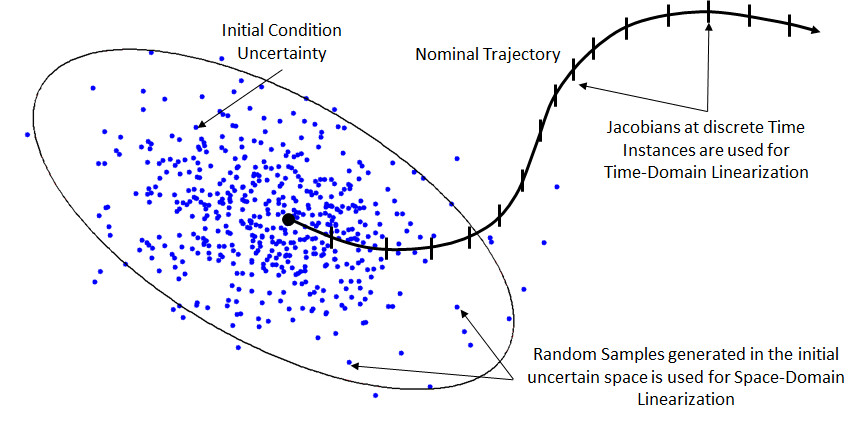
\includegraphics[width=\textwidth]{figures/FIG_3}
\caption{Setup for Time-Domain and Space-Domain Linearization}
\label{fig_lin}
\end{figure}

\subsection{Time-Domain Linearization}
\label{timedomain}

Let us consider the dynamical system given in Equation~\ref{nonlindiffeqn} with the initial condition $\textbf{x}_0$. We consider the nominal trajectory following the definition given in Equation~(\ref{gamma}) as $\gamma_{T,\mu_0}$, where $\mu_0 = E(\textbf{x}_0)$. The \textit{Time-Domain Linearization} considers multiple instances on the nominal trajectory, and the Jacobian of the system at those points. Together, a linear system matrix $A_{t}$ as in Equation~(\ref{lin_syst}) is formulated which uses the trajectory information $\gamma_{T,\mu_0}$ to approximate the actual nonlinear system for the given time interval $[0,T)$. Let us now look at the three methods that can be used for time-domain linearization. 

\underline{\textit{Method I: Average Jacobian:}} In this context, Surana \textit{et al.}~\cite{surana2012iterative} have used the \textit{time-average} of the Jacobian, given by:
\begin{equation}
\bar{J} = \frac{1}{T} \int_{0}^{T} J_t dt
\end{equation}
\noindent where,
\begin{equation}
J_t = \displaystyle \frac{\partial f(\mathbf{x})}{\partial \mathbf{x}} \bigg|_{\phi^t(\mu_0)}
\end{equation}
The weighted adjacency matrix and the graph Laplacian is found out using the definition of $\bar{J}$ instead of the Jacobian at a given point. The \textit{time-average} Jacobian is considered to be the vector field of the overall system with an idea that the Eigenvalues of the graph Laplacian from this system contains the inter-state connection information. 

However, it should be noted that one is ideally interested in the average Eigenvalues and the Eigenvectors of the Jacobian matrix. If the absolute values of the Jacobian are not taken, then one can often get wrong information of the system. Also, Eigenvalues and Eigenvectors of the time averaged Jacobian matrix does not correspond to the average Eigenvalues and Eigenvectors. For example, let us consider a system whose Jacobian at two different time instants are given as: 
\begin{equation}
\begin{array}{l}
A_{k} = \begin{bmatrix}
1.5 & -0.5 \\ -0.5 & 1.5
\end{bmatrix}
\hspace{5mm} A_{k+1} = \begin{bmatrix}
0.8 & 0.5 \\ 0.5 & 2.8
\end{bmatrix} \\
A_{k} + A_{k+1} = \begin{bmatrix}
2.3 & 0 \\ 0 & 4.3
\end{bmatrix}
\end{array}
\end{equation}
Clearly, the adjacency shows coupling effect between the two states at both the time instances, while the Eigenvectors of the matrix $A_k + A_{k+1}$ shows the states to be completely decoupled. Using this idea, the Eigenvalue and Eigenvector information of the adjacency or the Laplacian matrix is carried forward and is used to 
give the map $\psi$. Next, we discuss the two methods of clustering the states space, that do not utilize the \textit{time-averaged} Jacobian. The present methods instead record the inter-state connection information at each instance, carried forward by the Eigenvalues and the Eigenvectors of the Jacobian at each time instance.

\underline{\textit{Method II: Average Graph Laplacian:}} This method calculates the Eigenvalues $\lambda_{t_k}$ and Eigenvector $V_{t_k}$ of the $L_{t_k}$ matrix defined in~(\ref{graphlap}). At each point $\mathbf{x_t}$, the average Eigenvalues and the Eigenvectors are calculated using:
\begin{equation}
\begin{array}{cc}
\bar{\lambda} = \frac{1}{T} \int_{0}^{T} \lambda_t dt & \hspace{5 mm} \bar{V} = \frac{\int_{0}^{T} \lambda_t V_t dt}{\int_{0}^{T} \lambda_t dt} 
\end{array}
\end{equation}
Since, $L_{t_k}$ at any time instance, is a symmetric matrix, the \textit{Average Graph Laplacian} of the approximate linear system for the given time span $[0,T)$ is given as:
\begin{equation}
L^{T_s} = \bar{V} \bar{\lambda} \bar{V}^T
\end{equation}
The number of clusters and the cluster structure are derived using SC and Bayesian NMF.

\underline{\textit{Method III: Average Graph Adjacency:}} In this method, we find out the eigenvalues $\lambda'_{t_k}$ and the eigenvector $V'_{t_k}$ of the matrix $A_{t_k}$ defined in~(\ref{wead}). Next we find the \textit{time-averaged} $\lambda'_{t_k}$ and $V'_{t_k}$ using:
\begin{align}
&\bar{\lambda}' = \frac{1}{T} \int_{0}^{T} \lambda'_t dt 
&\bar{V}' = \frac{1}{T} \int_{0}^{T} V'_t dt  
\end{align}
Since $R_{t_k}$ at each time instant is a symmetric matrix, the \textit{Average Graph Adjacency} of the approximate LTIV system for the given time span $[0,T)$ is given by:
\begin{align}
A^{T_s} = \bar{V}'\bar{\lambda}'\bar{V}'^T
\end{align}

This graph adjacency information $A^{T_s}$ is used to obtain the cluster structure using SC and Bayesian NMF.

\underline{\textit{Averaging out Eigenvector Matrix for Weakly Connected Subsystems:}}
The Jacobian of any WCS in any instance has a block-diagonal matrix-like structure. The position of the bands, however, changes with time as shown in Figure~\ref{Eigenvect}. The pattern although shows discernible blocks, but they are permuted such that averaging over time can lead to erroneous interpretation. Thus, there is a need for proper orientation of the matrix, such that the blocks can be averaged and appropriately identified. An algorithm to correctly orient the Eigenvector matrices in a way that the blocks are easily identified is sketched next. The Algorithm~\ref{alg1} outlines the algorithm to generate a permutation matrix for such transformation of any given matrix $A$.

\begin{algorithm}[H]
\caption{To find out the permutation matrix for matrix $A$}
\label{alg1}
\begin{algorithmic}
\Require Square matrix $A$ 
\Ensure Permutation matrix $P$
\do Initialize $n$ as $size(A)$ \\
\do Initialize the Permutation Matrix $P$ as $abs(A)$ 
\For{$i = 1 \to n$} \\
\do find index $k$ of $max(P(i,:))$ \\
Assign $P(i,:) = 0$ \\
Assign $P(i+1:end,k) = 0$ \\
Assign $P(i,k) = 1$ 
\EndFor 
\end{algorithmic}
\end{algorithm}

\begin{figure}[H]
\centering
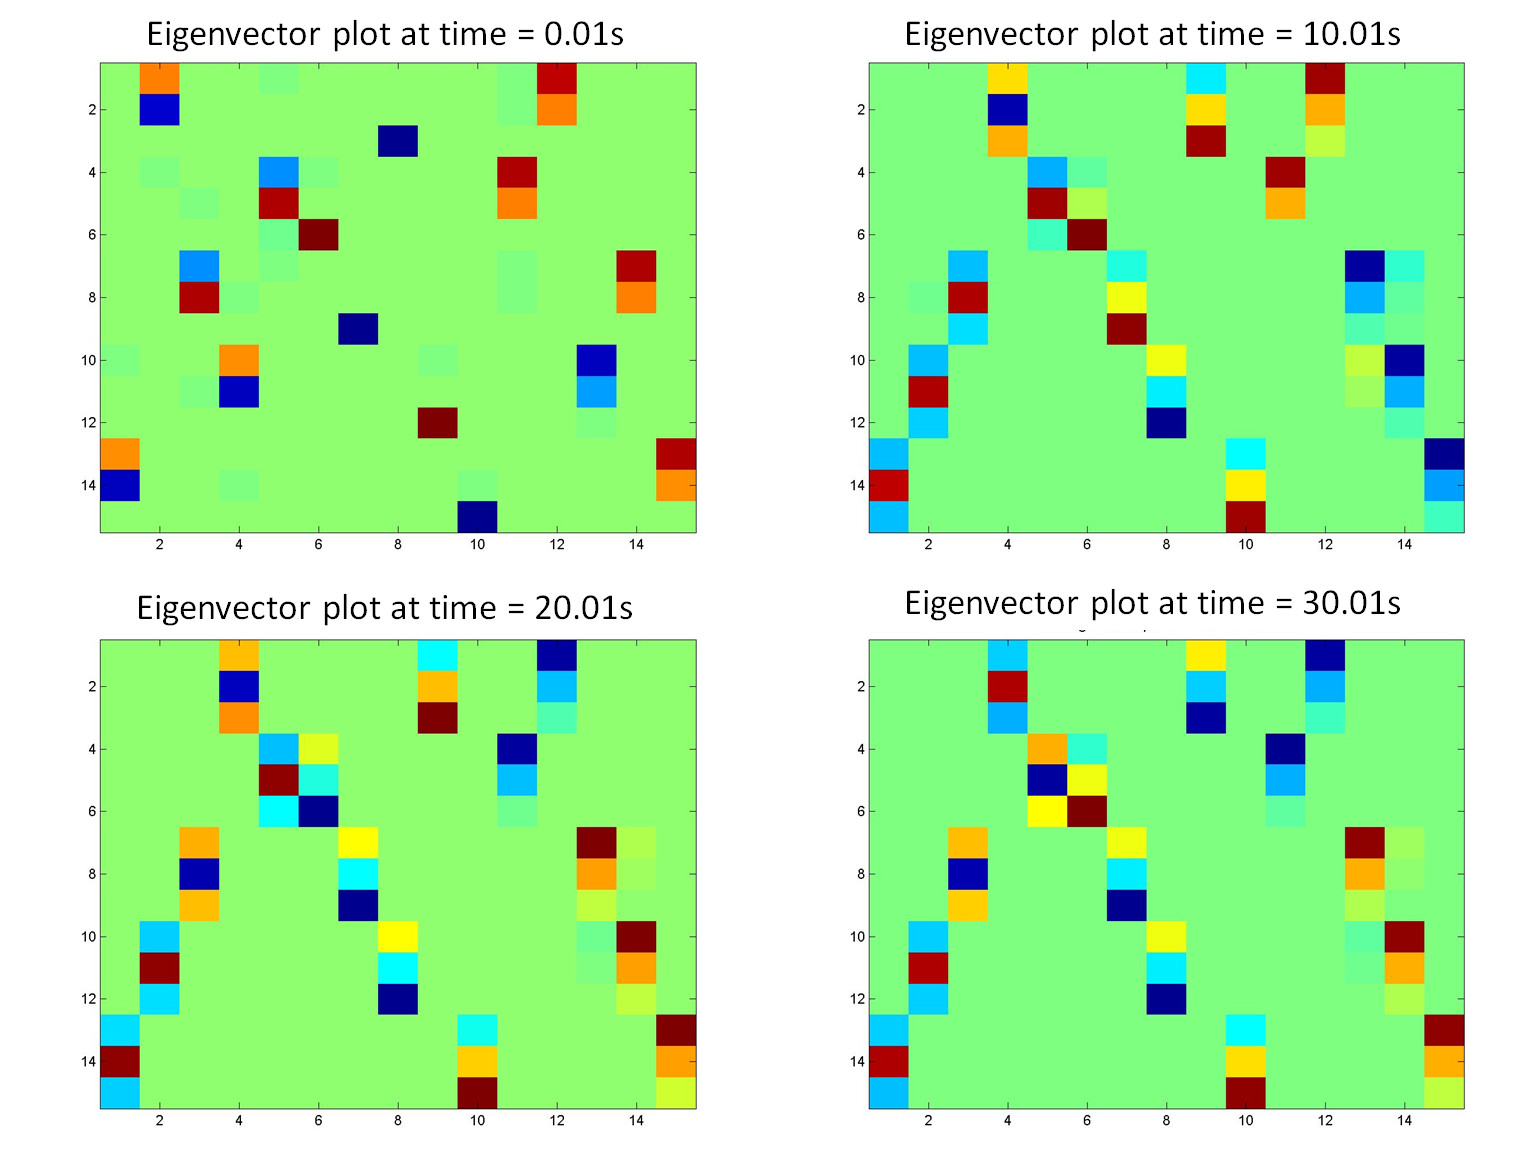
\includegraphics{figures/FIG_4}
\caption{Plot of Eigenvector Matrix of $W_t$ for a WCS at different time instance}
\label{Eigenvect}
\end{figure}

The motivation of the algorithm is to estimate a permutation matrix $P$, so that when it is multiplied with the Eigenvector matrix $W_t$, the resultant matrix has a block-diagonal structure. The algorithm begins with $P$ being initialized to $abs(A)$. Then, in each row of $P$, the element with the maximum value is identified. The component of the cell with the maximum value is assigned to 1 while the rest of the elements in the corresponding row and column are assigned to 0. By adopting this technique, one is guaranteed to obtain the permutation matrix that will give a block diagonal matrix when multiplied with the Eigenvector matrix. 

\begin{figure}[H]
\centering
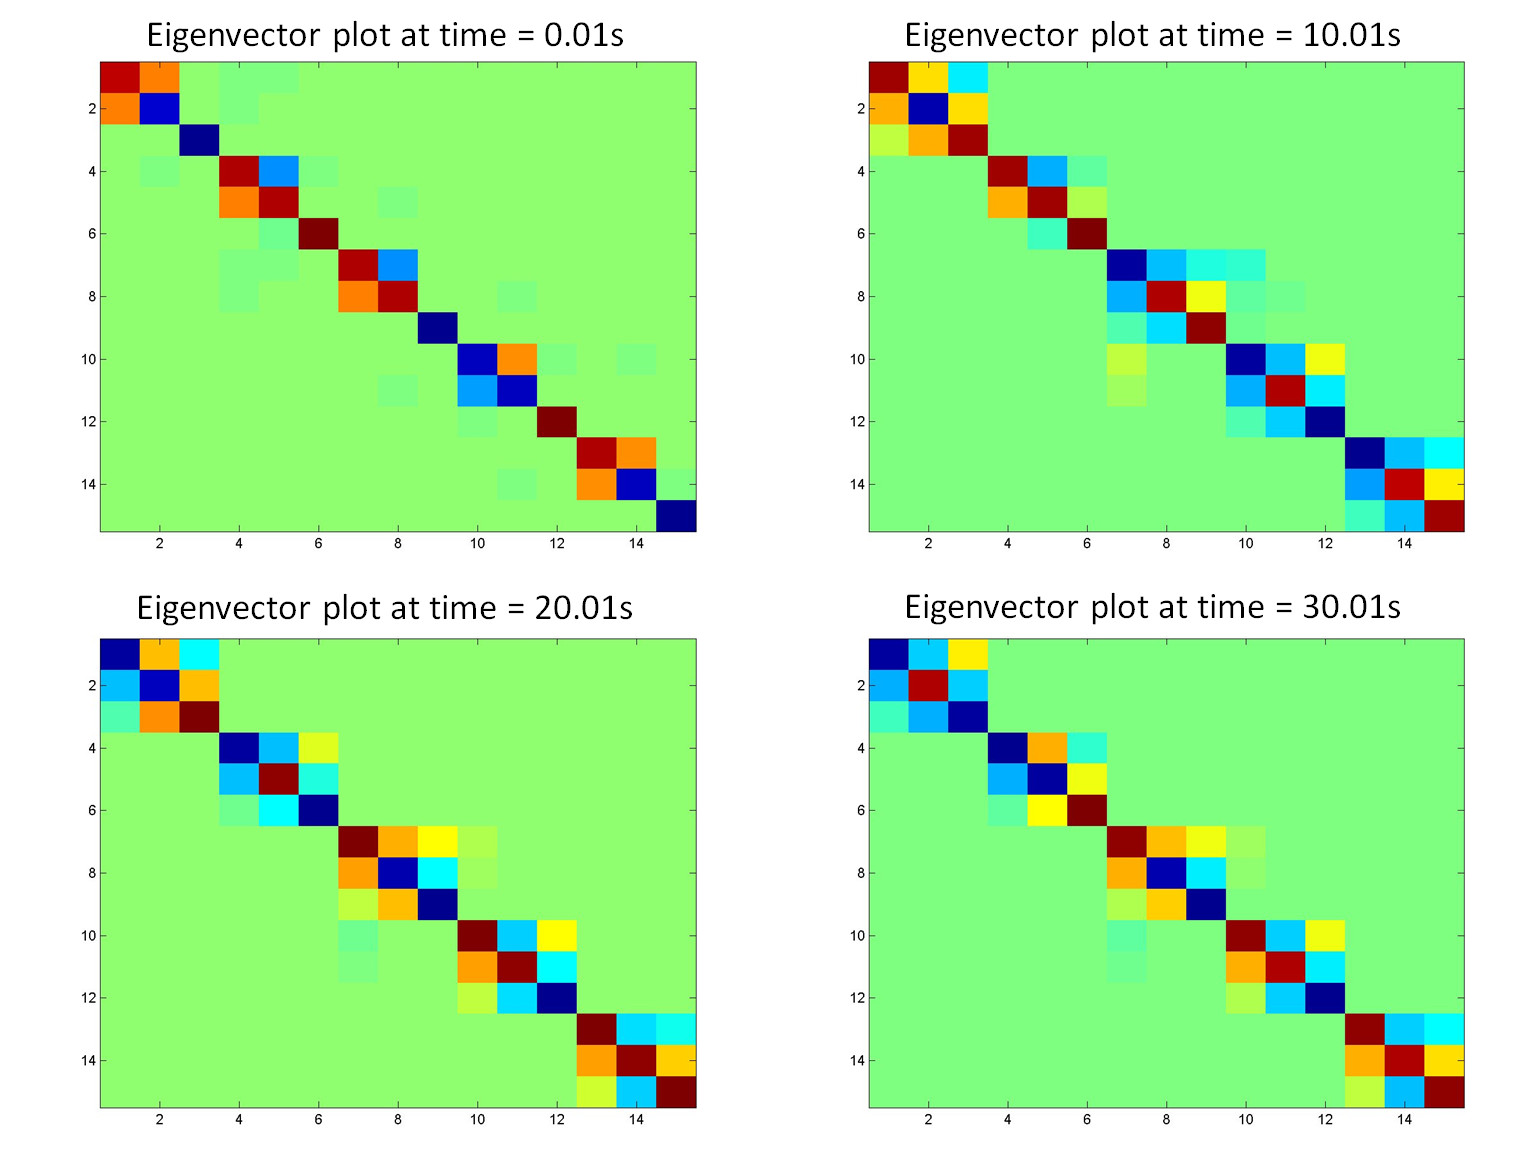
\includegraphics{figures/FIG_5}
\caption{Organized plot of Eigenvector Matrix of $W_t$ for a WCS at different time instance}
\label{Eigenvect2}
\end{figure}

The matrix $P$, once generated, can be used to determine the block matrix using $A_2 = A P^{-1}$. The given algorithm is valid only for decoupled or very weakly coupled oscillators. With increasing coupling strength, the Eigenvectors corresponding to the coupling function gets priority over the states, resulting in an improper result. The corresponding $A_2$ matrices for the Eigenvector matrices given in Figure~\ref{Eigenvect} are given in Figure~\ref{Eigenvect2}. Figure~\ref{Eigenvect2} shows the Eigenvector matrices when operated under the obtained permutation matrix. The figures indicate clear block-diagonal structures. This orientation facilitates easy averaging of the Eigenvector matrices. The corresponding positions of the Eigenvalues are also noted using the same permutation matrix. Thus, both the Eigenvector and the Eigenvalue information follows a continuous pattern throughout the time interval and their average lead to an interpretable information for the application of the clustering algorithm. Note that the block-diagonal structure shows more than the anticipated number of clusters at time t = 0, and then, the diagonal structure evolves with time. This behavior is nicely captured when the matrix is averaged out over time. 

\subsection{Space-Domain Linearization and Ergodicity}
\label{stat_lin_section}

In this section, the space-domain linearization method which, unlike the \textit{Time-Domain Linearization} techniques uses the initial condition uncertainty $\textbf{x}_0$, and not the nominal trajectory $\gamma_{T,\mu_0}$ is described.
Let us revisit the Taylor series expansion given in Equation~(\ref{taylor}). Given nonlinear function $f(\textbf{x})$ about a given point $\mu_t$ we obtain,
\begin{equation}
\label{jacobian}
f(\textbf{x}) = f(\mu_t) + Df(\mu_t) (\textbf{x} - \mu_t) + \mathcal{O} ||(\mathbf{x}  - \mu_t)^T(\mathbf{x}  - \mu_t)||
\end{equation}   
where, $\mu_t = E(\textbf{x}_t)$ and $Df(\mu_t)$ is the Jacobian of $f(\cdot)$ about $\mu_t$. Thus, the estimates of the linear model as in Equation~(\ref{linsyst}) are  computed as,
\begin{equation}
A_j = Df(\mu_t) \hspace{5 mm} b_j = f(\mu_t)
\end{equation}
The error due to such approximation is defined as,
\begin{equation}
\epsilon = f(\textbf{x}) - f(\mu_t) - Df(\mu_t) (\textbf{x} - \mu_t)
\end{equation} 
Hence, due to linearity of the operator $E(\cdot)$, the error can be calculated as $E \left[f(\textbf{x})\right] - f(\mu_t)$. The computed error can increase if $f$ is a highly nonlinear function. Topologically speaking, for all realization of $X(t,\omega) = w$, the trajectory $\phi^t(w)$ will be solved along the direction given by $Df(\mu_t)$ and not in the direction along $Df(w)$.
Other forms of linearization have been used in the past to simplify a nonlinear model. For example perturbation-based model~\cite{de2012efficient}, or Jacobian-based model~\cite{carbonell2007numerical,he2011enhanced,guardone2002roe} or more accurate approximation of nonlinear system~\cite{steeb1980non} linearizes the nonlinear system about a single point only. Therefore such existing methods suffer the same setback as described above. Also, while gradient-based methods need the knowledge of the exact Jacobian of the system, perturbation based method are highly sensitive to the amount of perturbation used. 

\underline{Statistical Linearization}: Spanos~\cite{roberts1986stochastic} suggested the technique of statistical linearization, by which a given nonlinear function $\textbf{x}_t$ of the random variable $\textbf{x}$ defined over $(\Omega,\mathcal{F},P_{\textbf{x}})$ can be approximated by a linear expression $\textbf{x}$. The approximate linearization of the function $f(\cdot)$ is given as,
\begin{equation}
\label{lin_model}
f(\textbf{x}_t) = b_{sl} + A_{sl}(\textbf{x}_t - \mu_t)
\end{equation}
Where,
\begin{equation}
\min_{A,b} J =  \int_{\Omega_t} ||f(z_t) - A_{sl}(z_t - \mu_t) - b_{sl} ||_2 p_{\textbf{x}_t} (z) dz 
\end{equation}
The system is much more accurate and has an expression of the exact solution and does not require the exact expression for the nonlinear velocity function and its Jacobian. The estimates of this model is given by the stationary solutions to the optimization problem, given as,
\begin{equation}
\label{stat_lin}
\begin{array}{rl}
\displaystyle \frac{\partial J}{\partial A_{sl}} = 0  & \Rightarrow  A_{sl} \; E[(\textbf{x}_t - \mu_t)^T (\textbf{x}_t - \mu_t)] - E[f(\textbf{x}_t - \mu_t)^T] = 0\\
& \Rightarrow A_{sl} = E[f(\textbf{x}_t - \mu_t)^T] P_{\textbf{x}_t \textbf{x}_t}^{-1} \\
\displaystyle \frac{\partial J}{\partial b_{sl}} = 0  & \Rightarrow b_{sl} - E[f] = 0\\
& \Rightarrow b_{sl} = E[f] 
\end{array}
\end{equation}

Such a linearization is \textit{Jacobian-free} and incorporates the information of the whole probability space, rather than just the mean of it. Figure~\ref{compare2} shows the difference in linearized matrix formulated by both Jacobian and Statistical Linearization from two different orientation of the $xyz$ axes. The schematic represents the approximation difference between the matrix formulated by either of the linearization technique and the Jacobian of the actual system about random samples generated in a given 2-D probability space. The $xy$ coordinates represent the state variables, while the $z$ axis shows the metric $||J_x - A||_2$, $x$ being a random sample. Figure~\ref{compare} shows the schematic difference in the behavior of the propagation of the linearized model against the actual nonlinear propagation. Since, the direction of trajectory for all points $\mathcal{X} \in \Omega$ can be very different from the trajectory for $\mathcal{X} = \mu_t$, the expected error in propagation for the Jacobian-based Linearized model can be very high. On the contrary, the Statistical Linearization minimizes this error. Hence, the trajectories for all $\mathcal{X} \in \Omega$ is expected to be approximated much better by the propagation $\dot{\textbf{x}}_t = A_{sl} \textbf{x}_t + b_{sl}$.

\begin{figure}[H]
        \centering
        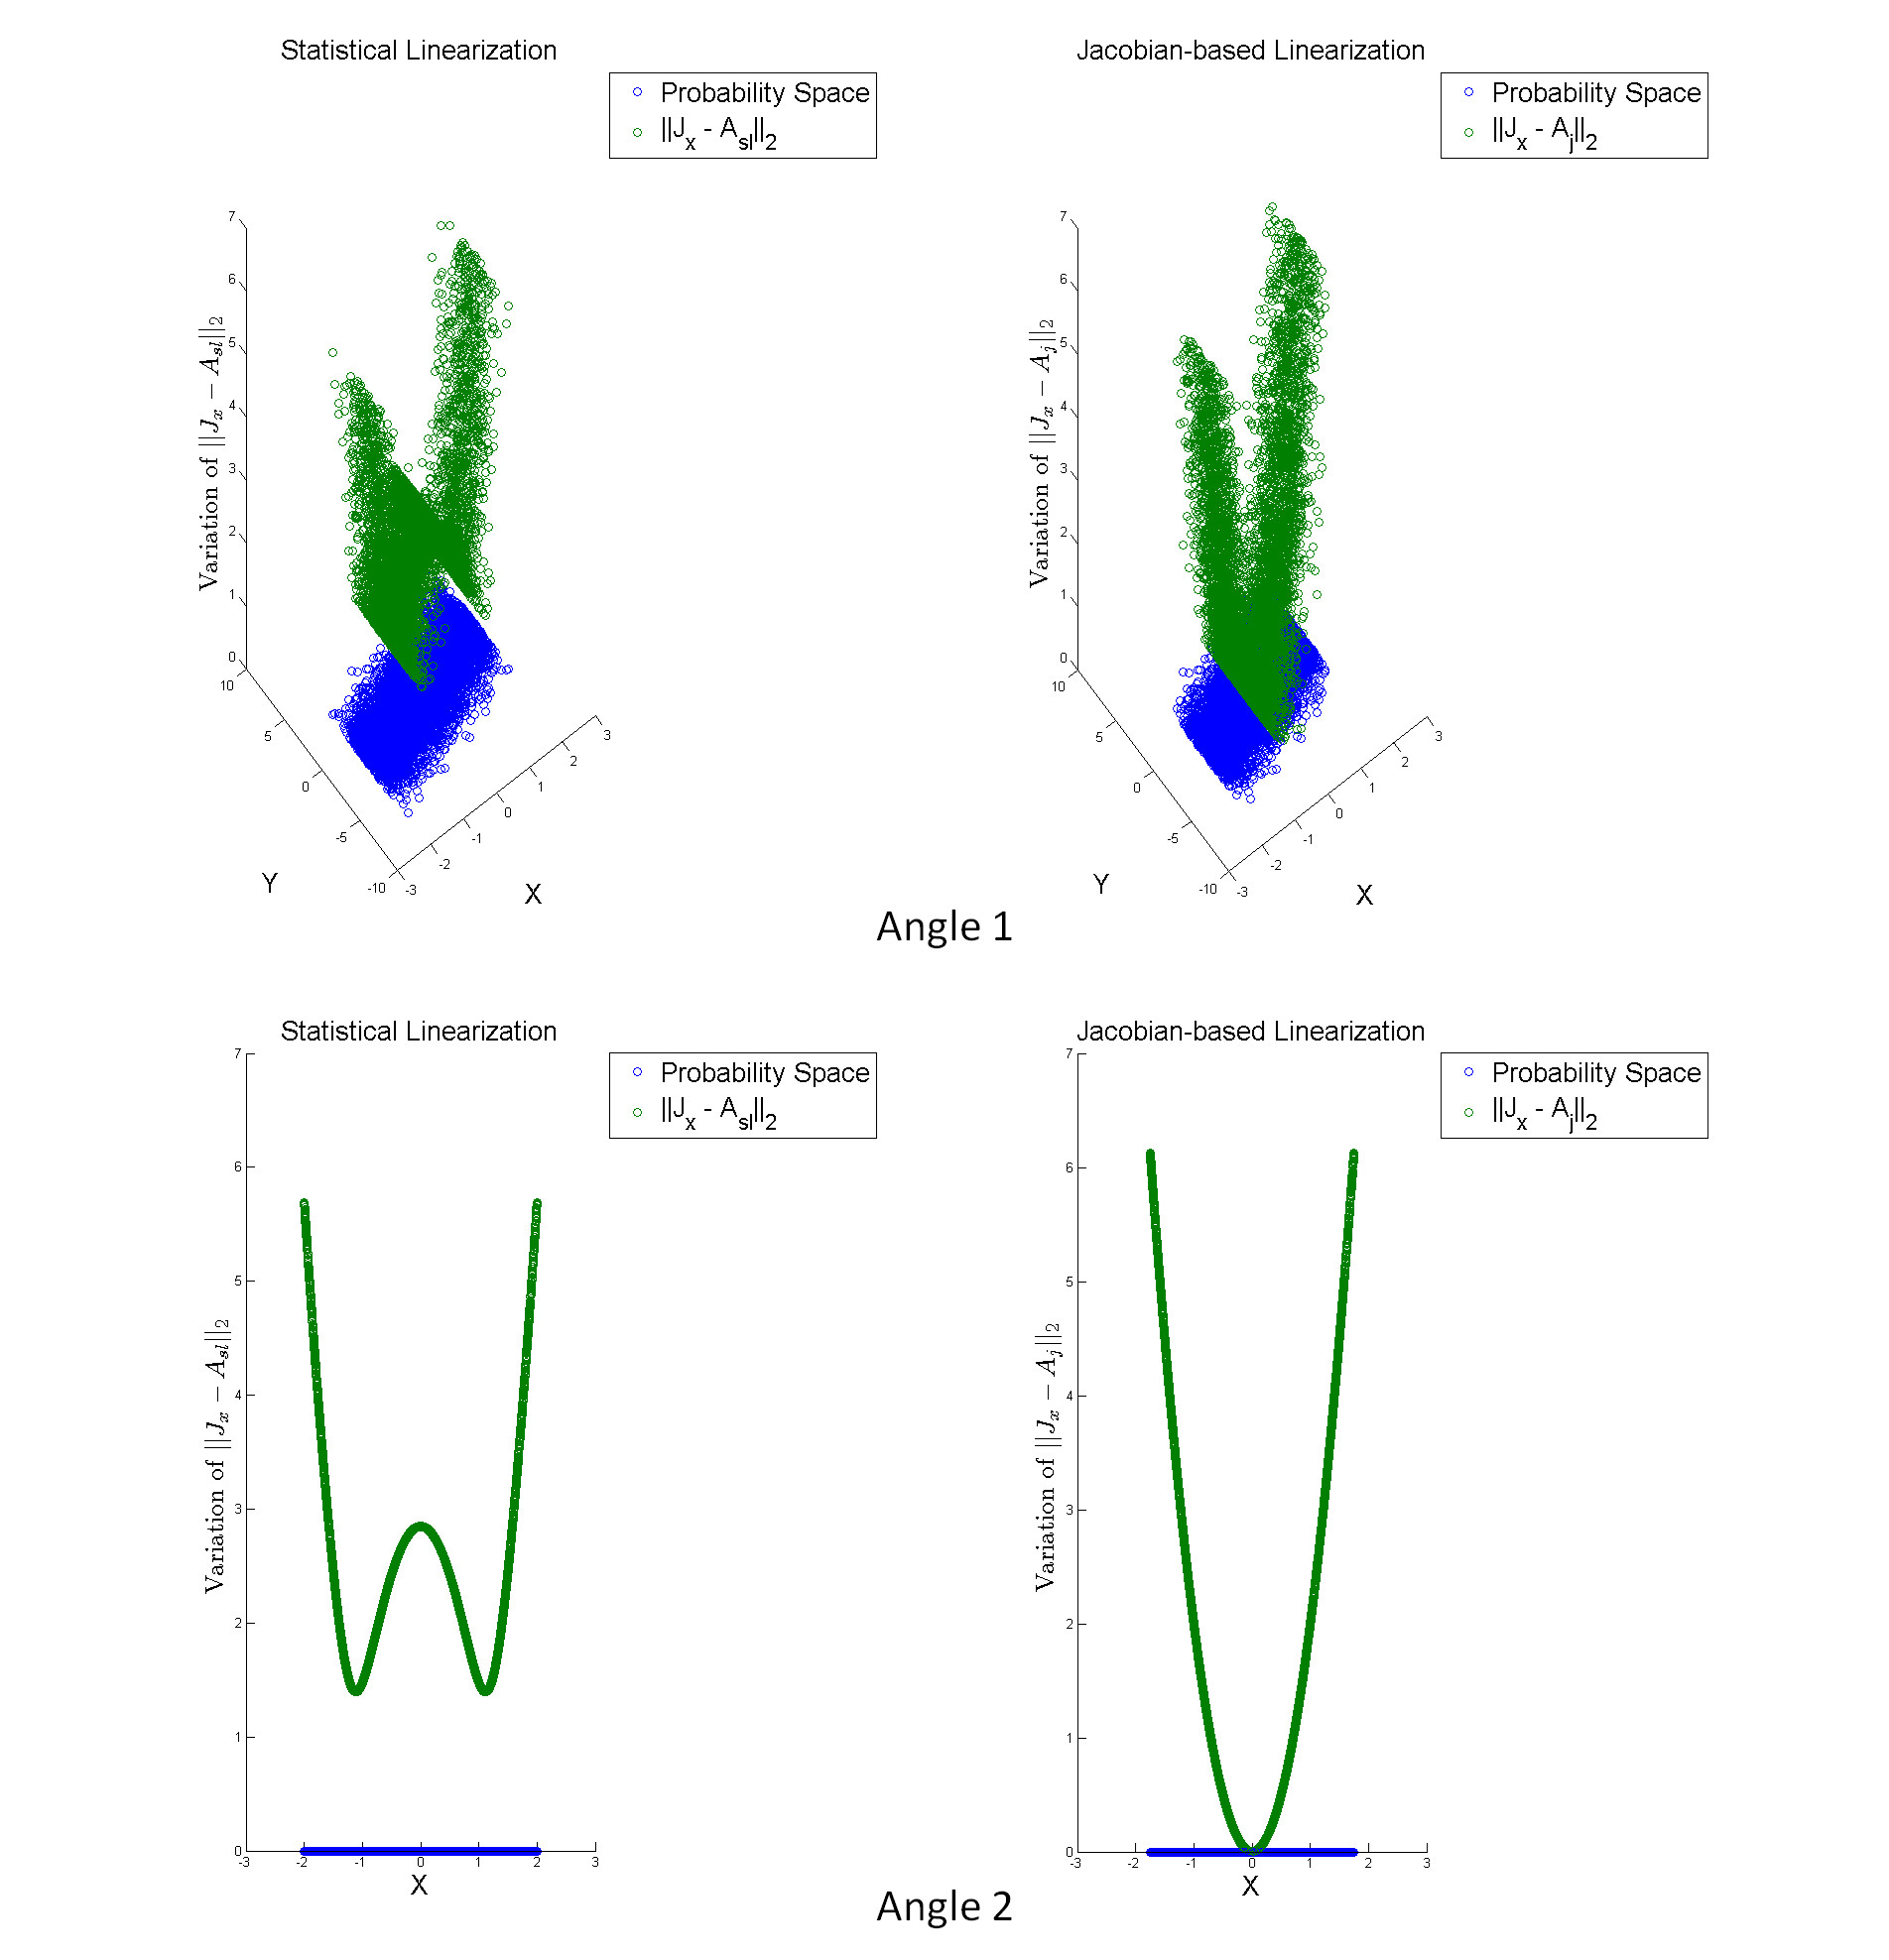
\includegraphics{figures/FIG_6}
        \caption{Comparison between Jacobian-based linearization matrix and Statistical linearization matrix}
        \label{compare2}
\end{figure}


\begin{figure}[H]
        \centering
        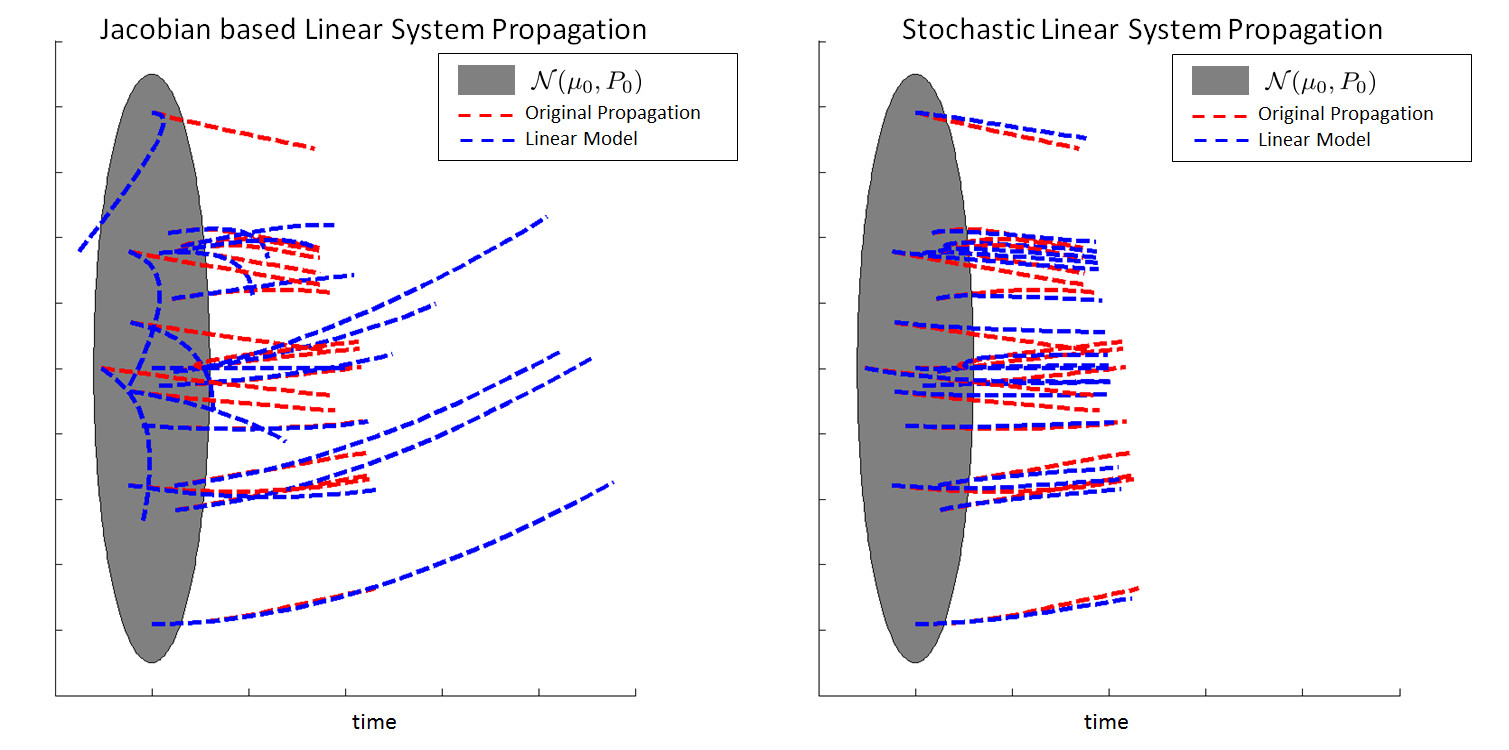
\includegraphics{figures/FIG_7}
        \caption{Comparison between propagation of Jacobian-based linearization and Statistical linearization}
        \label{compare}
\end{figure}

Let us now consider a nonlinear system defined by the equation $\dot{\textbf{x}}_t = f(\textbf{x}_t)$, with $\textbf{x}_t \sim \mathcal{N}(\mu_t,\sigma^2 I)$, $\textbf{x}_t \in \mathbb{R}^n$. The sigma points $\mathcal{X}$, the matrix $\mathcal{X} -\mu_t$ for $\textbf{x}_t$ and the corresponding weight vector will be given by the Equation~(\ref{sigmapt}) as,
\begin{equation}
\begin{array}{lcr}
\mathcal{X} = \begin{bmatrix}
\mu_t \\
\mu_t + \sigma  \lambda I_{n \times n} \\
\mu_t - \sigma \lambda I_{n \times n}
\end{bmatrix} &
\mathcal{X} - \mu_t =  \begin{bmatrix}
\textbf{0}_{1 \times n} \\
\sigma \lambda I_{n \times n} \\
- \sigma \lambda I_{n \times n}
\end{bmatrix}  &
 W = \begin{bmatrix}
\frac{\kappa}{\lambda^2}, \frac{1}{2\lambda^2}, \frac{1}{2\lambda^2}, \ldots , \frac{1}{2\lambda^2}
\end{bmatrix}^T_{1 \times (2n + 1)}
\end{array}
\end{equation} 
\noindent where, $\lambda = \sqrt{n+ \kappa}$. Any element $A_{{sl}_{ij}}$ of the Statistical Linearization matrix is thus given by the Equation~(\ref{stat_lin}) as,

\begin{equation}
\begin{array}{rl}
A_{{sl}_{ij}} = & \frac{1}{\sigma^2} \bigl[f_i(\mu_t)\cdot 0 \cdot W(0) + f_i(x_1 + \sigma \lambda,x_2,\ldots,x_n)\cdot 0 \cdot W(1) + \ldots \\
& + f_i(x_1 ,\ldots,x_j + \sigma \lambda,\ldots, x_n)\cdot \sigma \lambda \cdot W(j-1) \bigr.\\
& \left. + \ldots + f_i(x_1 ,\ldots,x_j - \sigma \lambda,\ldots, x_n) \cdot - \sigma \lambda \cdot W(j + n) \right] \\
= & \frac{f_i(x_1 ,\ldots,x_j + \sigma \lambda,\ldots, x_n) - f_i(x_1 ,\ldots,x_j - \sigma \lambda,\ldots, x_n)}{2 \sigma \lambda}
\end{array}
\end{equation}
\noindent With $\sigma \lambda \rightarrow 0$, the above expression of $A_{{sl}_{ij}}$ approaches the analytic expression for the derivative $\frac{\partial f_i}{\partial x_j}$. Hence, the Statistically linearized matrix $A_{sl}$ approximates the expression for the Jacobian $Df(\mu_t)$ for very low covariance values. 
 The Statistical Linearization is the only linearization technique among the rest, which can capture the contribution of both the vector field and the covariance information towards the coupling between the state variables. With high covariance values, the variation in $A_{sl}$ also increases. This behavior is not captured by any of the time-domain linearization methods. The method of Statistical Linearization will be referred to as SL in subsequent sections. 
 
Now, let us consider the initial probability space $(\Omega,\mathcal{F},P_{\textbf{x}_0})$ such that, $\phi:\Omega \rightarrow \Omega$ is a measure-preserving transformation. Since, $f$ is already a real-valued measurable function, hence by Birkhoff's Ergodic Theorem~\cite{Katok1995}, 

\begin{equation}
\lim_{n \rightarrow \infty} \frac{1}{n} \sum_{k=0}^{n-1} f \left( \phi^k (x) \right) = \int_{\Omega} f dP_{\textbf{x}_0}, \hspace{5 mm} x \in \Omega \text{ almost everywhere}
\end{equation}

\noindent which implies, that the space-domain average equals the time-domain average of the function $f$ for the nominal trajectory. Now, the above linearization techniques give us the formulation for the time average linearization $A_t$ and the state-space linearization $A_{sl}$. Thus, by property of ergodicity, we assume both the linearization to be equal. 

As discussed, the nonlinear system needs to be converted into a time-invariant linear model, where one can use the linear system matrix as a graph adjacency matrix.

\section{Non-overlapping Graph Clustering Methods}
\label{non_overlap_clustering}

The preliminary concept of clustering dates back to 1939~\cite{tryon1939cluster}. Clustering techniques and their comparisons are abundant. Domains like gene-clustering~\cite{eisen1998cluster,sturn2002genesis}, pattern recognition~\cite{bishop2006pattern,baraldi1999survey}, social media~\cite{lancichinetti2008benchmark}, image segmentation find abundant usage of data clustering techniques. Early reviews~\cite{cormack1971review,everitt1972cluster} mainly focused on heterogeneous datasets in which the affinity between the data points could be used to create groups of \textit{similar} and \textit{unlabeled} data objects. The research in clustering domain also focuses on measures to define the affinity, such that the number of groups of similar objects or \textit{clusters} can be increased. Researchers also have focused on the comparative study of different clustering algorithms such as hierarchical clustering, k-means clustering, Minimal Spanning Tree, and Fuzzy clustering~\cite{jain1988algorithms,jain1999data}. These reviews mainly focused on image segmentation and pattern recognition domains. The problems in these domains deal with a static dataset. Although the methods mentioned above are widely used even today on large datasets, these methods cannot be directly applied to our area of interest. The inapplicability of these existing clustering methods directly to the problem of WCS identification comes from the fact that such problem involves dynamics of the overall system. In dynamic system setting, the dataset is not static. 

For dynamic systems, one way to implement any clustering technique is to apply the clustering to the data at every time step. Another way to use a clustering technique to identify WCSs is to optimize the cluster structure in a way such that the error accumulated over the time is minimized. Both methodologies can be adopted only on a small dataset and for a short time. The curse of dimensionality in nonlinear systems is also tackled by finding a reduced order model~\cite{calinski1974dendrite,matthies2003nonlinear,wang2011two,carlberg2013gnat}. However, these methods are not useful in finding WCSs in large-scale systems. Kaneko~\cite{kaneko1990clustering,kaneko1990globally} studied clustering in a coupled nonlinear system. Kaneko studied coupled nonlinear models in the discrete-time scenario. The methods of detecting clusters are easy to implement. However, the applicability is limited to the specific type of problem discussed. Additionally, the presented methods cannot be used to study continuous time dynamic systems. The existence of cluster structure in coupled non-identical clusters has been reviewed by Lu \textit{et al.}~\cite{lu2010cluster}. They have shown that individual clusters under diffusive coupling can get fully synchronized if the coupling strength is high. The concept of Laplacian and Spectral Clustering has been introduced in this context~\cite{dellnitz2003congestion, varigonda2004graph}, and later has been studied for UQ in nonlinear dynamics~\cite{xia2011clustering,surana2012iterative, sorrentino2015complete}. 

Consider a linear system given by:
\begin{equation}
\label{lindiffeqn}
\dot{\mathbf{x}}_t = A \mathbf{x}_t + b
\end{equation}
The set of state variables $\textbf{x} \in \mathbb{R}^N$ are treated as vertices of a $N$-order undirected graph.  The association between each vertex is defined by the probability of transition between each state. At the end of the clustering, the subsets or the random vectors $\mathbf{y}_j$s are obtained. 
Such a system is easy to partition since the states are in a linear combination of each other. Standard methods such as PCA, POD, Factor Analysis, Jordan block decomposition and others. can be used to decompose the overall system. However, such methods either aim at finding a subspace of lower dimension or decouple the system using canonical coordinates. In the current work, our aim is slightly different and is focused on finding weakly or strongly connected subsystems, whose ensemble explains the dynamics of the overall large system.  

Let us consider a \textit{weakly coupled linear} system characterized by the matrix $A$. Decomposition of such a connected graph is based on the theory formulated by Fiddler~\cite{fiedler1973algebraic,fiedler1975property}, by which connectivity information is stored in the Eigenvalues and Eigenvectors of the adjacency matrix of a graph. The adjacency matrix can be written as~\cite{varigonda2004graph},
\begin{equation}
\label{adjcncy}
W = 0.5(P + P^T)
\end{equation}
where, $P$ is defined as,
\begin{equation}
\label{probmat}
p_{i,j} = | A_{ij} | /  \sum_{j=1}^n | A_{ij} |
\end{equation}
This transformation yields a matrix that stores the adjacency information of a weighted undirected connected graph. The transformation can also be interpreted from a probabilistic point of view. The matrix $A$ evidently stores information about the transition between state variables. This matrix $P$ is a (right) stochastic matrix as $p_{i,j} \ge 0$ for all $i,j$ and $\sum_j p_{i,j} = 1$ \cite{wolfowitz1963products}. Once, the $P$ matrix is obtained, the unique \textbf{stationary distribution} of $P$ (say $\pi_i$) or the left Eigenvector corresponding to the Eigenvalue of magnitude 1 is calculated. The stationary distribution is defined as, 
\begin{equation}
\pi_{j} =  \sum_{i \in S} \pi_i p_{ij} 
\end{equation}
Varigonda \textit{et al.}~\cite{varigonda2004graph} have used the following matrix definition as a graph adjacency matrix,
\begin{equation}
\label{wead}
W = MR = \frac{1}{2}(MP + (MP)^T)  \hspace{5 mm} M = diag(\pi_1,\pi_2,\ldots,\pi_n)
\end{equation}
where, the matrix $R$ is a reversible stochastic matrix given as~\cite{dellnitz2003congestion}: 
\begin{equation}
\label{revprobmat}
R = \frac{1}{2}(P + M^{-1} P^T M)
\end{equation}
A stationary Markov chain is said to be reversible if the transition matrix $R$ and the stationary distribution $\pi$ satisfies the following relation
\begin{equation}
\pi_i R_{ij} = \pi_j R_{ji}
\end{equation}
Under this transformation given in Equation~(\ref{revprobmat}), 
\begin{equation*}
\begin{array}{rl}
R_{ij} &= \frac{1}{2}\left(p_{ij} + \frac{1}{\pi_i}p_{ji}\pi_j \right) \\
\sum_j R_{ij} &= \sum_j \frac{1}{2}\left(p_{ij} + \frac{1}{\pi_i}p_{ji}\pi_j \right) \\
&= \frac{1}{2} + \frac{1}{2 \pi_i} \sum_j p_{ji} \pi_j = \frac{1}{2} + \frac{1}{2} =1
\end{array}
\end{equation*}
The following shows that $\pi_i'$s are also stationary transition probability distribution for $R$:
\begin{equation*}
\sum_i \pi_i R_{ij} = \frac{1}{2}\left[ \sum_i p_{ij} \pi_i + \pi_j \sum_i \pi_i \frac{1}{\pi_i} p_{ij} \right] = \frac{1}{2} \left(\pi_j + \pi_j  \right) = \pi_j
\end{equation*}
Thus, the adjacency matrix given by Equation~(\ref{adjcncy}) can be considered to be equivalent to a reversible matrix. Next, details related to several methods of graph clustering and their behaviors is outlined.


\subsection{Spectral Clustering}

Spectral Clustering (SC)~\cite{von2007tutorial} is a method of clustering a given graph using the spectrum or the Eigenvalue information. It uses a symmetric weighted adjacency matrix for clustering and obtains the Laplacian information from the given adjacency matrix. Given the adjacency matrix defined in Equation~\ref{wead}, the matrix can be decomposed into a set of well-connected components. By Matrix-Tree theorem~\cite{merris1994laplacian} $Rank(L) = n - w(G)$, whereby $L$ is the Laplacian of a binary adjacency matrix, $n$ is the order of matrix $A$, and $w(G)$ is the number of connected components. 
Graph Laplacian~\cite{merris1994laplacian,mohar1991laplacian} of $A$ is defined as:
\begin{equation}
L = D - W
\end{equation}
Where, $D$ is the degree matrix~\cite{bollobas1982graph}, and $W$ is the weighted adjacency matrix defined as in Equation~(\ref{wead}). Clearly, this matrix is both symmetric and positive semi-definite and one can trivially see that the lowest Eigenvalue is 0. For a weighted graph, the symmetric Graph Laplacian~\cite{chung1997spectral} is taken as:
\begin{equation}
\label{graphlap}
L = I - D^{-1/2} W D^{-1/2}
\end{equation}
The above formulation results from the minimization of the normalized cut objective function for clustering a given weighted adjacency graph~\cite{shi2000normalized}. Besides, the transformation serves the purpose of scaling down the matrix by its adjacency, which makes the analysis to be much easier. The properties of symmetry and positive semi-definite remains intact, and additionally it has other properties such as:
\begin{itemize}
\item $0 \leq \lambda_i \leq \sqrt{2}$
\item $\sum_i \lambda_i \leq n$, with the equality holds when there is no isolated vertex. 
\item $\lambda_1 =0, \lambda_{n-1} \geq \frac{n}{n-1} $
\end{itemize} 

Figure~\ref{fig:spectral} shows a schematic of the SC methodology. Given an adjacency matrix (Figure~\ref{fig:sc_adjacency}), one computes the eigenvalue of the normalized graph Laplacian as in Equation~\ref{graphlap} (Figure~\ref{fig:sc_eigen}). From the eigenvalue plot, one decides the cluster structure from the eigenvector matrix corresponding to number of zero eigenvalues (Figure~\ref{fig:sc_cluster}).

\begin{figure}[H]
\centering
\begin{subfigure}{0.32\textwidth}
\centering
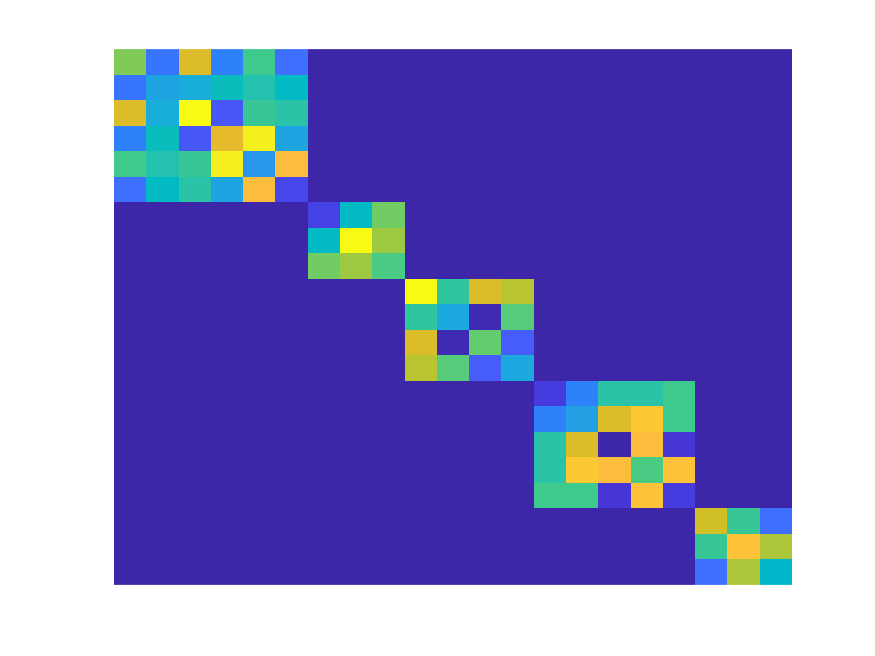
\includegraphics[width=\textwidth]{figures/adjacency}
\caption{}
\label{fig:sc_adjacency}
\end{subfigure}
\begin{subfigure}{0.32\textwidth}
\centering
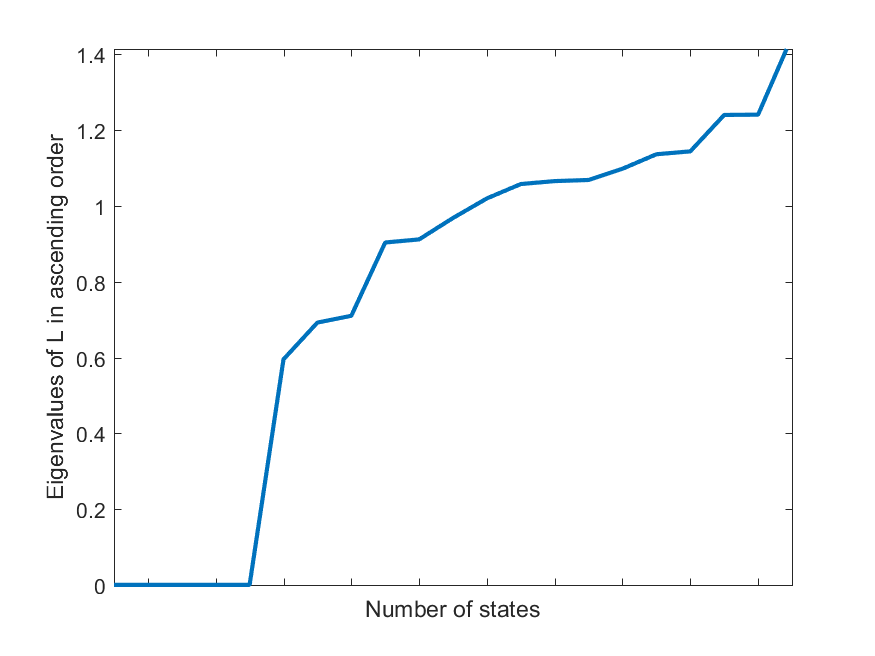
\includegraphics[width=\textwidth]{figures/eig}
\caption{}
\label{fig:sc_eigen}
\end{subfigure}
\begin{subfigure}{0.32\textwidth}
\centering
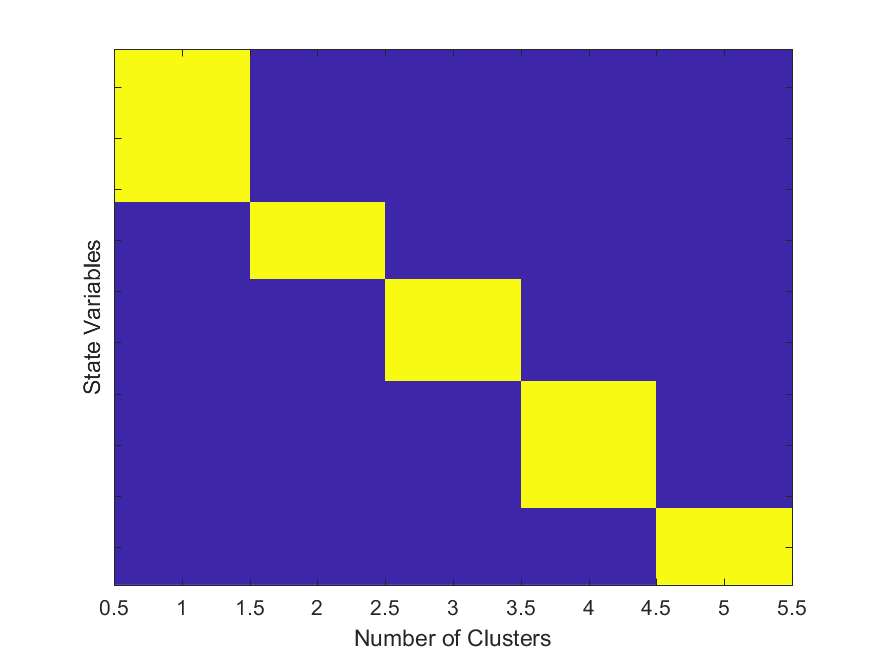
\includegraphics[width=\textwidth]{figures/cluster}
\caption{}
\label{fig:sc_cluster}
\end{subfigure}
\caption{Schematic of Spectral Clustering: (a) shows a typical adjacency matrix comprising of discernible blocks (b) shows the eigenvalue plot of the symmetric normalized Laplacian for the corresponding adjacency and (c) shows the cluster structure derived from the eigenvector of the corresponding zero eigenvalues}
\label{fig:spectral}
\end{figure}



This method is essentially used to identify clusters in a Block-Diagonal Matrix of the form 
\begin{equation}
\label{block}
A = \bigoplus_{i=1}^m A_i = \begin{bmatrix}
A_1 & 0 & \ldots & 0 \\ 0 & A_2  & \ldots & 0 \\ \vdots & \vdots & \ddots & \vdots \\  0 & 0 & \ldots & A_m
\end{bmatrix}
\end{equation}
For a fully connected graph $A_j$, the corresponding stochastic matrix $P_j$ will have exactly one Eigenvalue with magnitude 1, and the symmetric graph Laplacian $L_j$ will have exactly one Eigenvalue of magnitude 0. The graph Laplacian of a block-diagonal adjacent matrix also takes the form of a block diagonal matrix as,
\begin{equation*}
L_{sym} = \bigoplus_{i=1}^m L_i = \begin{bmatrix}
L_1 & 0 & \ldots & 0 \\ 0 & L_2  & \ldots & 0 \\ \vdots & \vdots & \ddots & \vdots \\  0 & 0 & \ldots & L_m
\end{bmatrix}
\end{equation*}
The Eigenvalue plot for the Laplacian gives us the number of clusters, which is approximately equal to Number of \textbf{almost zero} Eigenvalues. Sometimes an Eigenvalue plot becomes too ambiguous in terms of finding the correct point that refers to the highest \textit{almost zero} value. Even a naked eye judgment fails to take such decision. Hence a `knee point' algorithm has been adopted~\cite{salvador2004determining}, that finds out the point of maximum curvature of the Eigenvalue plot, by estimating a pair of straight lines that best describes the plot. 


\subsection{Non-negative Matrix Factorization}

Non-negative Matrix Factorization (NMF) (earlier formulated as Positive Matrix Factorization~\cite{paatero1994positive}) belongs to the class of problem, whereby a given matrix $A \in \mathbb{R}^{n \times m}_+$ is factorized as
\begin{align}
W = XY
\end{align}  
Where, the resultant factor matrices are $X \in \mathbb{R}^{n \times p}_+$ and $Y \in \mathbb{R}^{p \times m}_+$, and $P$ is the right stochastic matrix defined in Equation~(\ref{probmat}). The factorization can be done in such a way such that, $p \ll n $ and $p \ll m$. Pioneering research in this field has been conducted by Lee and Seung~\cite{lee1999learning}. They have solved a simple least square formulation to get the update equations for $X$ and $Y$. 

Since then, NMF has been a subject of immense interest and have been found to be very useful in Graph Clustering, Data storage, and Community Detection.
Ding \textit{et al.} have shown that the symmetric NMF (i.e., where $W$ is symmetric, and $X = Y$) is similar to kernel k-means and Spectral Clustering~\cite{ding2005equivalence}. Wang \textit{et al.}~\cite{wang2011community} have used the symmetric NMF to detect community in an interconnecting network. Wang \textit{et al.} have formulated a problem of factorizing a symmetric graph adjacency matrix as,
\begin{align}
\min_{\hat{X} \geq 0}  \bigg| \bigg| W - \hat{X}\hat{X}^T \bigg| \bigg|_{F}^2
\end{align}
where, the resultant factor matrix $\hat{X}$, is normalized. After normalization, each element corresponds to the probability of occurrence of an element in the community. A  Probabilistic approach to NMF has been adopted by Zass and Shashua~\cite{zass2005unifying}. Bayesian framework has been adopted by Virtamen \textit{et al.}~\cite{virtanen2008bayesian} and later by Schmidt \textit{et al.}~\cite{schmidt2009bayesian} and are shown to be better performing than existing algorithms. However, a key question about the ideal value of $p$ to enable the clustering, has been addressed experimentally. Psorakis \textit{et al.}~\cite{psorakis2011overlapping} have proposed a Probabilistic Graphical framework, to capture the probability of the existence of a particular element in a community and to iteratively decide the smallest possible value of $p$, such that the error $\min_{\hat{X} \geq 0}  \bigg| \bigg| W - \hat{X}\hat{X}^T \bigg| \bigg|_{F}^2$ is minimized. The Bayesian NMF uses a probabilistic graphical model given in Figure~\ref{bnmf}.  

\begin{figure}[H]
\centering
\tikzstyle{block} = [circle, draw, fill=blue!20, 
    minimum size=.5cm, text centered, minimum height=4em]
\tikzstyle{line} = [draw, -latex']
\begin{tikzpicture}
\node [block] (A) {$\beta_k$};
\node [block, left of=A,yshift=-2cm,xshift=-1.5cm] (B) {$a$};
\node [block, left of=A,yshift=2cm,xshift=-1.5cm] (C) {$b$};
\node [block, right of=A,yshift=2cm,xshift=1.5cm](D){$X_{ik}$};
\node [block, right of=A,yshift=-2cm,xshift=1.5cm](E){$Y_{kj}$};
\node [block, right of=D,yshift=-2cm,,xshift=1.5cm](F){$W_{ij}$};
\path [line] (B) -- (A);
\path [line] (C) -- (A);
\path [line] (A) -- (D);
\path [line] (A) -- (E);
\path [line] (E) -- (F);
\path [line] (D) -- (F);
\end{tikzpicture}
\caption{Probabilistic Graphical Model for the Bayesian NMF framework}
\label{bnmf}
\end{figure}

As per Figure~\ref{bnmf}, $X \in \mathbb{R}^{n \times l}_+$ and $Y \in \mathbb{R}^{l \times n}_+, l<n$ are matrices, which are estimated from the Bayesian model,

\begin{equation}
\begin{array}{ll}
p(W,H,\beta|P) =& \displaystyle \frac{p(W|X,Y,\beta)p(X|\beta)p(Y|\beta)p(\beta)}{p(P)} \\
& \propto p(P|X,Y,\beta)p(X|\beta)p(Y|\beta)p(\beta)
\end{array}
\end{equation}
Where, $P_{ij}$'s have a prior Poisson distribution, with the mean as $P_{ij} = \sum_k X_{ik} Y_{kj}$. $X_{ik}$ and $Y_{kj}$ are i.i.d random variables, with $X_{ik},Y_{kj} \sim \mathcal{HN} (0,\beta_k^{-1})$. The estimates $\hat{X}$ and $\hat{Y}$ are obtained by maximizing the log-likelihood of the posterior function. At the end of the posterior update, the number of clusters is determined by the minimum rank $l$ of the matrix $X$. The values of $X$ and $Y$ gives the quantification of the participation of a particular state in a cluster. Since in our case, $W$ is a symmetric matrix, $X$ is equal to $Y$. For a fully connected graph $P$, the value of $k$ after the Bayesian update comes out to be 1. Hence, in a block-diagonal matrix as in Equation~(\ref{block}), the value of $l$ equals $m$.  

\subsection{Comparison of SC and NMF}

Now, the similarities and the dissimilarities in the theory and application of both the methods of clustering is elaborated. Ding \textit{et al.} observed that the objective function from the normalized cut algorithm, which gives rise to the formulation of the symmetric Graph Laplacian, can also lead to the formulation for symmetric NMF. In other ways, the objective function for symmetric NMF, $\min_{\hat{X} \geq 0} \bigg| \bigg| W - \hat{X}\hat{X}^T \bigg| \bigg|_{F}^2$, with some orthogonality constraint for $X$, gives rise to the formulation for SC. Theoretically, under the required conditions, both the methods are expected to return the same results for a block diagonal matrix. However, further analysis of the two methods gives rise to following points of dissimilarities:

\begin{enumerate}
\item  For SC, it is important to have a symmetric, positive semi-definite weighted graph adjacency. NMF can work on any matrix $A$ with all $A_{ij} \ge 0$.
\item  SC requires the Eigenvalue information, and the number of clusters is decided from the Eigenvalue plot. Calculating Eigenvalues for a large matrix can be computationally expensive. Also, the detection of the cluster structure in case of SC depends on the usage of the knee-point algorithm, which uses a threshold for detecting the number of clusters. Thus, the cluster structure can be ambiguous. On the other hand, NMF does not require the Eigenvalue information. The model estimates are computed from a Bayesian update equation, and at the end of the update, the number of clusters is automatically decided by the rank of the estimated matrix.
\item Given a matrix $A$, with no proper discernible blocks (for example, a fully populated matrix), NMF is not expected to show any cluster. With SC, one can still obtain a cluster structure if the number of clusters is specified. 
\item SC results in non-overlapping clusters. Even in an overlapping adjacency matrix, SC will detect disjoint sets, because of the application of k-means clustering at the last step of the SC algorithm. NMF provides the degree of participation of a particular state in a cluster, that can be used to identify overlapping clusters. The clustering idea applied in NMF can be applied to SC too, for obtaining overlapping clusters with a degree of participation. 
\end{enumerate}


% \subsection{Louvain Modularity Maximization}


% \begin{equation}
% Q = \frac{1}{2m_q} \displaystyle \sum_{i,j} \left[W_{i,j} - \frac{k_i k_j}{2m_q} \right] \delta(c_i, c_j)
% \end{equation}

% \noindent where, $m_q = \sum_{i,j}W_{i,j} = N/2$, $k_i = \sum_i W_{i,j}$ and $c_i$ is the partition to which $i^{\text{th}}$ state belongs. The delta function $\delta(c_i,c_j)$ is 
% \begin{equation}
% \delta(c_i,c_j) = \begin{cases}
% 1 & c_i = c_j \\ 0 & \text{otherwise}
% \end{cases}
% \end{equation}
% Maximizing $Q$ gives the values of $c_i$'s, $i = 1$ to $N$ and hence determines the cluster structure. In the next section, the adjacency matrix and the identified cluster structure will be detailed.   



Let us now look into the method of UQ, and how the above method of linearization and clustering can benefit any UQ methodology.




\section{Clustering and Filtering}
\label{method}
%In interconnected systems, despite detecting the WCSs, it is highly probable that the clustered model should give errors in the approximation of the mean and covariance of the overall system, as the identified subsystems are propagated individually, ignoring the inter-cluster coupling strength. 
The UQ in the clustered model is effective only for a short period of time. Due to the coupling effect, the cluster structure may change after some initial propagation. In this section, the method of solving a stochastic dynamical system with uncertainty in the initial condition is discussed. Measurements or observations are available for the system at a different time. The solution involves periodically updating the cluster structure with the availability of a measurement. The measurement is hypothesized to improve the cluster structure. The updated clustered model based on measurement can be more effective in approximating the solution of the system and subsequently filtering out the noise. The steps used are as follows:

\begin{enumerate}
\item Given the problem 
\begin{equation}
\label{meas_eqn}
\begin{array}{lr}
\dot{\textbf{x}}_t = f(\textbf{x}_t) & \textbf{x}_{t_0} = \textbf{x}_0 \\
\textbf{z}_t = \textbf{x}_t + \nu
\end{array}
\end{equation}
Where, $\textbf{z}_t$ is the measurement at a given time, and $\nu \sim \mathcal{N}(0,R_{\textbf{z}})$ is the measurement error.
\item At a time $t_k$, the linearized model is formulated as, 
\begin{equation}
f(\textbf{x}_{t_k}) = A_{sl}\textbf{x}_{t_k} + b_{sl}
\end{equation}
\item The state space $\textbf{x}_t \in \mathbb{R}^n$ is clustered into subsystems as $\lbrace \mathbf{y}_1, \mathbf{y}_2 , \ldots , \mathbf{y}_m \rbrace$ following the Spectral Clustering or NMF methodology explained in Section~\ref{non_overlap_clustering}.
\item Each subsystem $\dot{\textbf{y}} = f(\textbf{y})$  is propagated parallel to each other using any highly efficient UQ method as discussed in Chapter~\ref{chap:uq}. At the end of the propagation the predicted mean and covariance are obtained as $\mu_{k+1|k}$ and $P_{k+1|k}$
\item Let us consider an observation $\textbf{z}_{t_k + h}$ available at time $t_k + h$. The steps involving filtering out the noise follows the well-known Kalman Filtering technique.
\item The innovation covariance is then computed as,
\begin{equation}
P_{\nu \nu} = R_{\textbf{z}} + P_{k+h|k+h-1}
\end{equation}
\item The cross correlation matrix is computed as $P_{k+h|k+h-1}$
\item The Kalman gain is computed as, 
\begin{equation}
K = P_{k+h|k+h-1} P_{\nu \nu}^{-1}
\end{equation}
\item The measurement update is carried out,
\begin{equation}
\begin{array}{l}
\mu_{k+h|k+h} = \mu_{k+h|k+h-1} + K(\textbf{z}_{t_k + h} - \mu_{k+h|k+h-1})  \\
P_{k+h|k+h} = P_{k+h|k+h-1} - K P_{\nu \nu} K^T
\end{array}
\end{equation}
\item After the Filtering, the mean and covariance values are re-calibrated. Using the velocity function and the uncertainty information available after time $t_k + h$, the system is again linearized using the techniques explained in Section~\ref{wcs:linearization}. The cluster structure is recomputed using the linearized matrix following the methodologies explained in Section~\ref{non_overlap_clustering}. Further analysis is done following the steps 4-9 in an iterative manner.
\item The corrected mean and covariance of the whole system is collected for given time instances at the end of the iteration.
\end{enumerate}

This problem setup is a simple case involving simple measurement equation and additive measurement noise. More realistic problems can be addressed by varying the measurement equation and also by including process noise in the state space equation. The filtering technique needs to be adjusted accordingly, and the problem can be solved. However, the critical idea of improving the recomputing and improving the cluster structure with the availability of noise remains the same. 

In subsequent sections, some numerical experiments are performed to identify the most suitable method of linearization and clustering. The WCS-based UQ method will be used to solve the filtering problem discussed above.

\section{Numerical Experiment}
\label{wcs:num_exp}
This section describes the numerical experiments on two standard scalable nonlinear dynamical system test problems consisting of weakly coupled oscillators. In each problem, it is desired to decompose the state space using the seven methods listed in Table~\ref{techniques}, and propagate random samples through the clustered nonlinear model for a given time $[t_0,t_0 + T_s]$ to see the effectiveness of the decomposition methods. For each system, the number of oscillators (and hence the dimension) $N$ and a coupling parameter $e$ in the equation have been varied. The value of $N$ is varied randomly from 5 to 50 with three levels, while the coupling factor $e$ is varied from 0 (decoupled) to 0.1(highly coupled) at seven levels. The experiment uses the four Methods of Linearization as discussed in Section~\ref{wcs:linearization} and two Methods of Clustering as discussed in Section~\ref{non_overlap_clustering}. It is to be noted that Method II of linearization completely depends on the concept of Laplacian only. Hence, it is not compatible with the Bayesian NMF clustering technique. Hence, the experiments have been carried out with following seven techniques listed in Table~\ref{techniques}.

\begin{table}[H]
\centering
\caption{Techniques of Linearization and Clustering}
\label{techniques}
\resizebox{\textwidth}{!}{  
\begin{tabular}{|c|c|c|c|c|c|c|}
\hline 
Technique I & Technique II & Technique III & Technique IV & Technique V & Technique VI  & Technique VII  \\ 
\hline 
Method I + SC & Method II + SC & Method III + SC & Method I + NMF & Method III + NMF  & SL + SC & SL + NMF\\ 
\hline 
\end{tabular} 
}
\end{table}

  Thus, the three Linearization and two Clustering techniques together form a single factor named `Linearization and Clustering' with five levels. The factors and their type and levels are described in Table~\ref{factors}. Each numerical experiment is performed with 1000 replications. 

\begin{table}[H]
\centering
\caption{Factors and levels of experiment}
\label{factors}
\begin{tabular}{|c|c|c|}
\hline 
Factor & Type & Levels \\ 
\hline 
Type of Problems & Random & 2 \\ 
\hline 
$n$ & Random & 7 \\ 
\hline 
$e$ & Random & 8 \\ 
\hline 
Linearization and Clustering & Fixed & 7 \\ 
\hline 
%Clustering & Fixed & 2 \\ 
%\hline 
\end{tabular} 
\end{table}


 The time-space is discretized with an increment of $\bigtriangleup t$. Given a random sample $x_0 \in \mathbb{R}$ of the random variable $\mathbf{x}_0 \sim \mathcal{N}(\mu_0, \Sigma_0)$, the sample point has been propagated with the help of the original system defined in Equation~(\ref{stochdyn}) to obtain $x_t$ and also the clustered model defined in Equation~(\ref{substochdyn}) to obtain $x_t^c$. An experiment has been designed to test the effect of the methods of linearization and the methods of clustering. The error in propagation is defined as 
 
 \begin{equation}
e_{\textbf{x}}(t_k) = \bigg|\bigg| \frac{\textbf{x}_{t_k} - \textbf{x}^c_{t_k} }{ \textbf{x}_{t_k} }\bigg|\bigg|_2 
\end{equation}
Where, $|| \cdot ||_2$ is the $L^2$ norm. The time averaged error is calculated as $\bar{e}_{\textbf{x}} = \frac{1}{T} e_{\textbf{x}}(t_k)$. Lower the value of this metric, higher is the efficiency of the linearization and clustering method.  


\subsection{Linear System}
\label{linear_system}

To test the proposed methodology, first a linear system is taken up as an example. Let us consider the equation for the system of $n$ informed agents~\cite{xia2011clustering} defined as,
\begin{equation}
\label{lin_syst}
\begin{array}{l}
\dot{x}_i = -x_i + a_i + \epsilon_i \displaystyle \sum_{j=1}^N g_{ij} x_j \hspace{5 mm} i = 1 \text{ to } n
\end{array}
\end{equation}
As per the definition of linear system given in Equation~(\ref{lindiffeqn}), the linear system matrix is given as.
\begin{equation}
A = -\textbf{I} + \epsilon G
\end{equation}
The system comprises of $m$ subsystems that are diffusively coupled with the neighboring states. Each subsystem has $n_m$ states with $\sum_{i} n_m = n$. For each subsystem, $a_i = a_m$ and $\epsilon_i = \epsilon_m$ for all $i = 1$ to $n_m$. Figure~\ref{linsyst} shows a 10-dimensional system comprising of $m = 3$ decoupled subsystems. Each subsystem with $n_1 = 4$, $n_2 = 3$ and $n_3 = 3$, state variables are coupled with each other. Thus, the $G$ matrix (as shown) is a block-diagonal matrix. 

\begin{figure}[H]
        \centering
        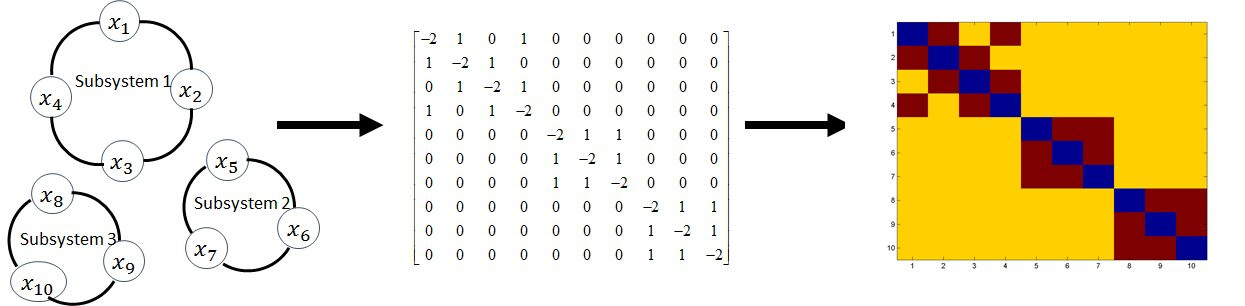
\includegraphics[width=\textwidth]{figures/FIG_10}
        \caption{Example of 10-dimensional informed agent system. The system comprises of subsystems of 3-4 states which are diffusively coupled}
        \label{linsyst}
\end{figure}

\begin{figure}[H]
        \centering
        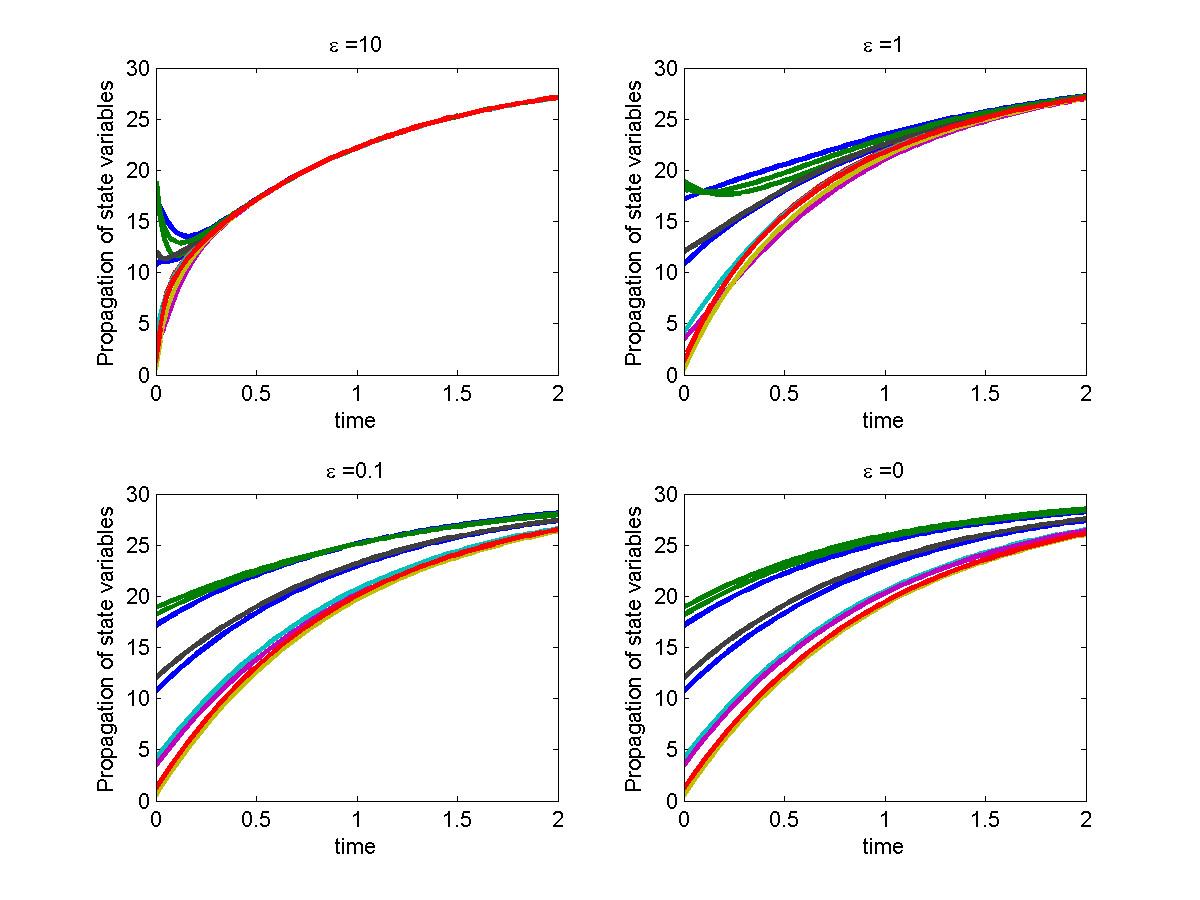
\includegraphics[width=\textwidth]{figures/FIG_11}
        \caption{Propagation of 10-dimensional coupled system with different values of $\epsilon$}\label{linsysts}
\end{figure}

However, the final $A$ matrix structure will depend on the value of $\epsilon$. While high value of $\epsilon_i$ will enforce the coupling between the oscillators, a very low value of $\epsilon$ will allow the algorithm to identify the system as a set of decoupled oscillators. The steady state solution of the individual states with $\epsilon = 0$, is $x_i^* = a_i$. The steady state solution for the whole system is given by,
\begin{equation}
\textbf{x}^* = -A^{-1}a = -(\epsilon G - \textbf{I})^{-1}a
\end{equation}

The sum of each row of $A$ is -1. Hence, an Eigenvalue of $A$ and $A^{-1}$ is -1. The corresponding Eigenvector is the null-space of the matrix $G$, which is $\textbf{1}_{n \times 1}$. Thus, the state solution for the system is also $\textbf{x}^* = a$.
Let us check the propagation of a 10-dimensional system, that is fully coupled with no subsystem present, under different values of $\epsilon$ and $a = 30\cdot\textbf{1}_{n  \times 1}$. Figure~\ref{linsysts} shows the propagation of the coupled 10-dimensional system with the same initial condition. It is seen that the system becomes almost completely \textit{synchronized} with a high value of $\epsilon$. As the value decreases, the \textit{phase-locking} also vanishes and the states behave as if they are decoupled. The value of $\epsilon$ controls the rate at which the states reach the steady-state solution. 

Next, the assemblies of different subsystems have been taken up to form large systems of higher order. The clustering techniques on the systems have been applied to identify the decoupled subsystems. The identified cluster structure does not depend on the time interval or the initial condition uncertainty. Hence, there is no need to apply the linearization techniques. The dimension of the overall system, the number of subsystems, and the number of clusters (or subsystems) identified by the two clustering techniques are given in Table~\ref{linsyst_table}. 

\begin{table}[H]
\centering
\scriptsize{
\caption{Dimension of overall system, number of subsystems, and the number of clusters identified by the different clustering techniques}
\label{linsyst_table}
\begin{tabular}{|c|c|c|c|c|c|c|c|}
\hline 
\multirow{2}{*}{$n$} & $m$ & $m$ & $m$ & \multirow{2}{*}{$n$} & $m$ & $m$ & $m$ \\ \cline{2-4} \cline{6-8} 
& Expected & with SC & with NMF & & Expected & with SC & with NMF \\ \hline
20    &    5    &    5    &    5    &    200    &    50    &    50    &    50    \\ \hline
30    &    7    &    7    &    7    &    300    &    75    &    75    &    75    \\ \hline
40    &    10    &    10    &    10    &    400    &    100    &    100    &    100    \\ \hline
50    &    12    &    12    &    12    &    500    &    125    &    125    &    125    \\ \hline
60    &    15    &    15    &    15    &    600    &    150    &    150    &    150    \\ \hline
70    &    17    &    17    &    17    &    700    &    175    &    175    &    175    \\ \hline
80    &    20    &    20    &    20    &    800    &    200    &    200    &    200    \\ \hline
90    &    22    &    22    &    22    &    900    &    225    &    225    &    225    \\ \hline
100    &    25    &    25    &    25    &    1000    &    250    &    250    &    250    \\ \hline
\end{tabular}
} 
\end{table}

The values show that both the clustering methods are equally efficient in identifying the correct number of subsystems. However, the efficiency in finding out the right cluster structure is not evident from these values. 

\begin{figure}[H]
        \centering
        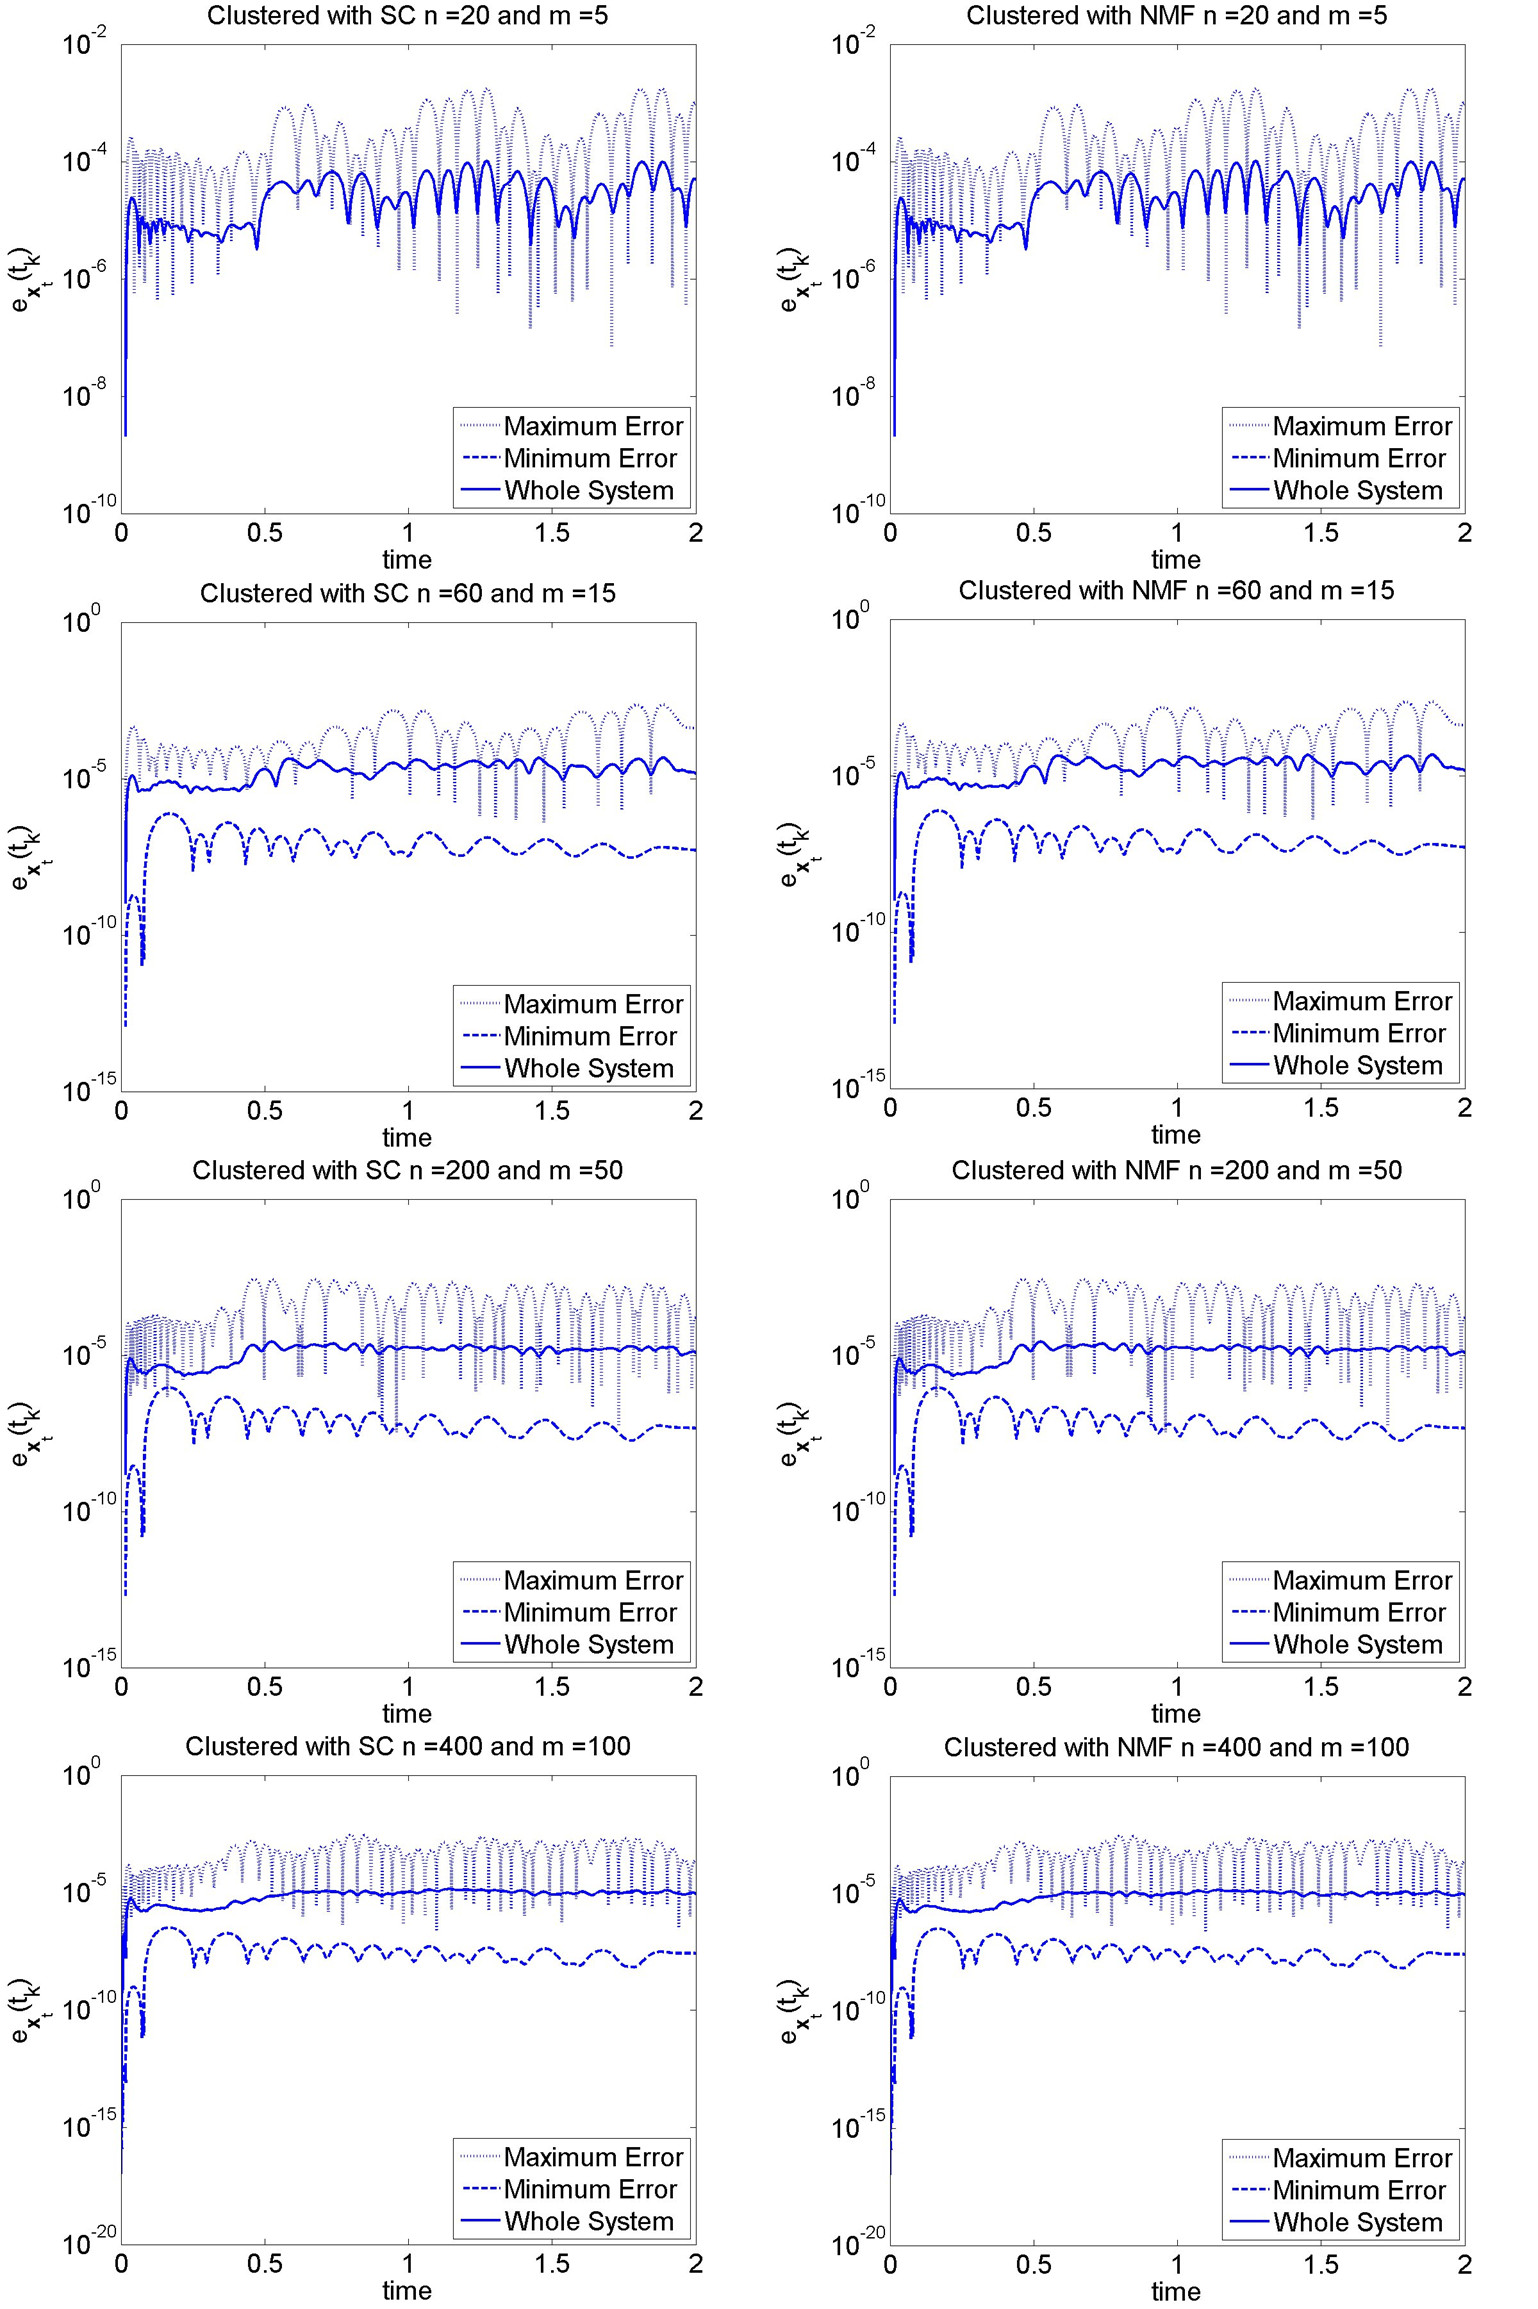
\includegraphics[width=\textwidth,height=\textwidth]{figures/FIG_12}
        \caption{Propagation of the coupled linear system for different size of problems}
        \label{linsyst_prop}
\end{figure}

Next, some random initial conditions have been taken up and used to propagate both the original system and the clustered model obtained by the two clustering methods. The comparison of the trajectory gives us a clear idea about the accuracy of the clustering methods. Figure~\ref{linsyst_prop} shows the plot of error in propagation in terms of $e_\textbf{x}(t_k)$ vs time of the linear system for different dimensions. For each system we have calculated the time-averaged error for each of the cluster as $\bar{e} = \int e_\textbf{x}(t_k) dt_k$. The `Maximum Error' and the `Minimum Error' plot corresponds to the error propagation plot for those clusters with the maximum and minimum values of $\bar{e}$. It can be observed that with $n = 20$, the minimum error value for a cluster is 0. The error range for the whole system is between $10^{-7}$ and $10^{-4}$. The error range for the system is fairly constant for different dimensions of the problems. Also, there is no such discernible variation in the error for the `Maximum Error' and the `Minimum Error' plots for the different problems. This observation speaks of the robustness of the method of clustering to the size of the problem. 

\subsection{Weakly Coupled Van der Pol Oscillators}
Let us consider the second order differential equation of $N$ nonidentical and decoupled unforced Van der Pol oscillators~\cite{van1920theory} given as, 
\begin{equation}
\ddot{x}_i - \nu_i (1-x_i^2) \dot{x} + x_i = 0
\end{equation}
with a nonlinear damping function controlled by a single parameter $\nu_i$ and linear stiffness. The state space  formulation can be written as,
\begin{equation}
\label{weak_vanderpol}
\begin{array}{l}
\dot{x}_i = y_i + \epsilon (x_{i-1} - 2x_i + x_{i+1}) \\
\dot{y}_i = \nu_i(1-x_i^2)y_i - x_i  
\end{array}\hspace{5 mm} i = 1,2,\ldots,N
\end{equation}
The undamped equation of this model represents the equation of a simple harmonic oscillator, while a positive value of $\nu_i$'s forces the individual systems to enter into a limit cycle oscillation. Analysis shows that, $x_i = [0 \; 0]^T$ is an unstable equilibrium point. Let us now study the behavior of the system under Statistical Linearization for a system with $\epsilon = 0$, $N = 5$ with random value of mean $\mu = [0.2, 0.2, \ldots, 0.2]$ and covariance $ \alpha \Sigma$, where 
\begin{equation}
\Sigma = \begin{bmatrix}
1 & 0.1 & 0.1 & 0.1 & 0.1 & 0.1 & 0 & 0 & 0 & 0 \\
0.1 & 1 & 0.1 & 0.1 & 0.1 & 0.1 & 0 & 0 & 0 & 0 \\
\vdots & \vdots & &  & \ddots & & \ddots    & & \vdots & \vdots \\
0 & 0 & 0 & 0 & 0 & 0 & 0.1 & 0.1 & 1 & 0.1 \\
0 & 0 & 0 & 0 & 0 & 0 & 0.1 & 0.1 & 0.1 & 1 \\
\end{bmatrix}
\end{equation}
\noindent The time-dependent linearization technique is independent of the value of $\alpha$. To show the change in Statistically linearized matrix $A_{sl}$, the value of $\alpha$ is varied. Figure~\ref{statlinsysts} shows the color image of $A_{sl}$ computed using different values of $\alpha$. The plot shows that the matrix $A_{sl}$ is capable of capturing the effect of the covariance values. With higher values of $\alpha$, the two different blocks of the covariance matrix is captured by the matrix $A_{sl}$. Intuitively, it can be inferred that, the time-based linearization is unable to capture these blocks. Next, we take up several such initial conditions for the purpose of further experimentation. The system has been linearized and the state space has been decomposed based on each of the initial conditions and the dynamics of the system. Table~\ref{weakvanderpol} shows the average mean and covariance of error in propagation obtained for the seven methods for some of the test cases. All the methods consistently show low error values for all of the test cases. A few percentage of the error values are in the range of $10^{-1}$, while maximum error values are in the range of $10^{-7}$ or $10^{-10}$. There is a need of a detailed statistical analysis so as to get a deeper insight into the test results. 

\begin{figure}[H]
        \centering
        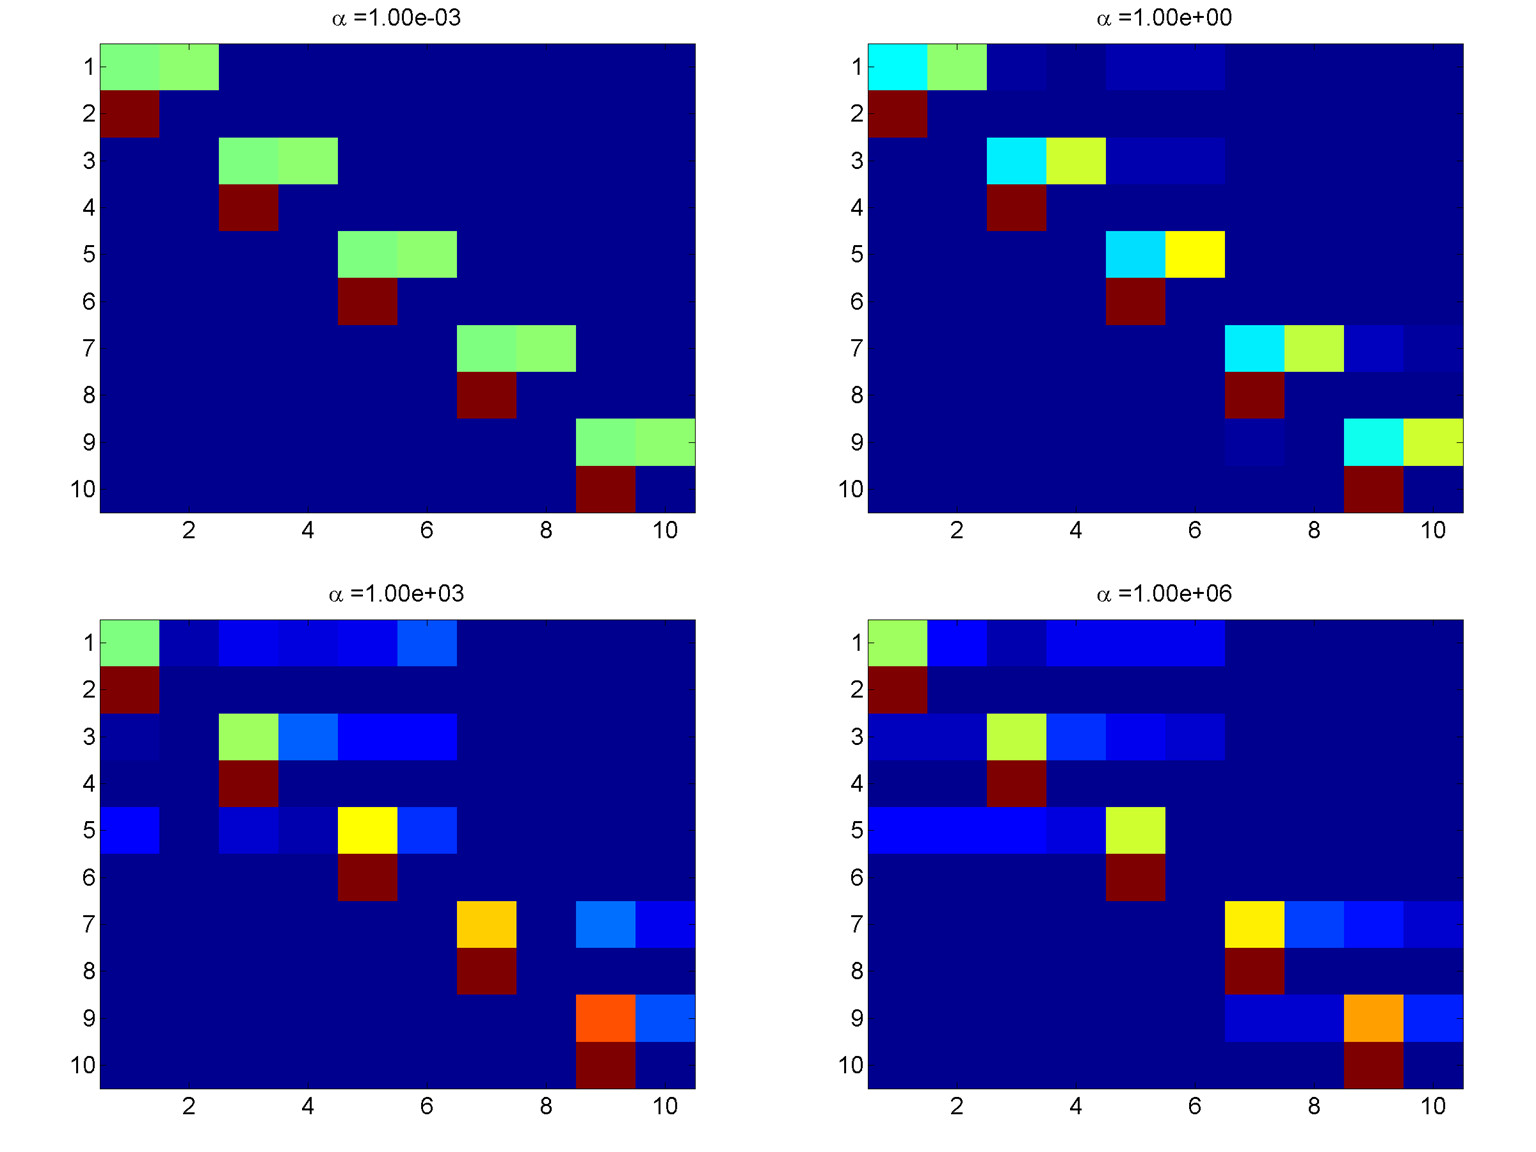
\includegraphics[width=\textwidth]{figures/FIG_13}
        \caption{Variation in $A_{sl}$ of 10-dimensional coupled oscillator system with different values of $\alpha$}
        \label{statlinsysts}
\end{figure}

\begin{table}[H]
\caption{RMS \textit{time-averaged} mean and \textit{time-averaged} covariance for different test setups in Weakly Coupled Van der Pol Oscillators}
\begin{center}
\resizebox{\columnwidth}{!}{
\label{weakvanderpol}
\begin{tabular}{|c|c|c|c|c|c|c|c|c|c|c|c|c|c|c|c|}
\hline 
\multirow{2}{*}{$n$} & \multirow{2}{*}{$e$} &  \multicolumn{2}{c|}{Method I}  & \multicolumn{2}{c|}{Method II} & \multicolumn{2}{c|}{Method III} & \multicolumn{2}{c|}{Method I} & \multicolumn{2}{c|}{Method III} & \multicolumn{2}{c|}{SL} & \multicolumn{2}{c|}{SL} \\ \cline{3-16}
                        &                         & \multicolumn{2}{c|}{ + SC}     &   \multicolumn{2}{c|}{ + SC}    &    \multicolumn{2}{c|}{ + SC}    &   \multicolumn{2}{c|}{ + NMF}  &  \multicolumn{2}{c|}{ + NMF}  & \multicolumn{2}{c|}{ + SC}  &  \multicolumn{2}{c|}{ + NMF} \\ \hline
10    &    0.00E+00    &    4.88E-02    &    6.22E-02    &    4.80E-02    &    6.18E-02    &    4.88E-02    &    6.22E-02    &    4.70E-02    &    6.13E-02    &    4.71E-02    &    6.13E-02    &    1.18E-06    &    3.56E-04    &    4.75E-02    &    5.96E-02    \\ \hline
10    &    1.00E-01    &    2.48E-02    &    4.28E-02    &    2.57E-02    &    4.71E-02    &    2.48E-02    &    4.28E-02    &    2.77E-02    &    5.58E-02    &    2.71E-02    &    5.07E-02    &    2.48E-02    &    4.28E-02    &    3.21E-02    &    5.71E-02    \\ \hline
10    &    1.00E-02    &    2.34E-02    &    4.15E-02    &    2.46E-02    &    4.63E-02    &    2.34E-02    &    4.13E-02    &    2.65E-02    &    5.33E-02    &    2.62E-02    &    5.25E-02    &    2.34E-02    &    4.14E-02    &    3.01E-02    &    5.62E-02    \\ \hline
10    &    1.00E-03    &    6.18E-02    &    6.49E-02    &    5.89E-02    &    6.09E-02    &    5.42E-02    &    5.29E-02    &    6.11E-02    &    6.56E-02    &    6.00E-02    &    6.56E-02    &    5.42E-02    &    5.29E-02    &    5.98E-02    &    6.53E-02    \\ \hline
10    &    1.00E-04    &    5.30E-02    &    6.53E-02    &    5.01E-02    &    6.09E-02    &    4.70E-02    &    5.39E-02    &    5.17E-02    &    6.49E-02    &    5.24E-02    &    6.50E-02    &    4.71E-02    &    5.37E-02    &    5.32E-02    &    6.52E-02    \\ \hline
10    &    1.00E-05    &    5.01E-02    &    6.52E-02    &    4.83E-02    &    6.13E-02    &    4.60E-02    &    5.72E-02    &    4.96E-02    &    6.47E-02    &    5.00E-02    &    6.49E-02    &    4.41E-02    &    5.16E-02    &    4.98E-02    &    6.43E-02    \\ \hline
10    &    1.00E-06    &    4.24E-02    &    6.09E-02    &    4.13E-02    &    5.86E-02    &    4.19E-02    &    5.99E-02    &    4.17E-02    &    6.06E-02    &    4.23E-02    &    6.06E-02    &    3.78E-02    &    4.86E-02    &    4.42E-02    &    6.14E-02    \\ \hline
10    &    1.00E-07    &    4.45E-02    &    6.15E-02    &    4.33E-02    &    5.93E-02    &    4.44E-02    &    6.14E-02    &    4.36E-02    &    6.11E-02    &    4.41E-02    &    6.11E-02    &    3.90E-02    &    4.93E-02    &    4.52E-02    &    6.22E-02    \\ \hline
20    &    0.00E+00    &    6.36E-05    &    6.56E-03    &    6.35E-05    &    6.56E-03    &    6.36E-05    &    6.56E-03    &    8.69E-05    &    7.03E-03    &    7.51E-05    &    6.60E-03    &    1.01E-04    &    6.84E-03    &    6.08E-05    &    6.53E-03    \\ \hline
20    &    1.00E-01    &    2.13E-07    &    2.73E-06    &    1.03E-02    &    1.54E-02    &    6.34E-02    &    5.99E-02    &    3.03E-02    &    4.12E-02    &    2.15E-02    &    3.57E-02    &    3.49E-09    &    8.75E-08    &    2.67E-02    &    3.84E-02    \\ \hline
20    &    1.00E-02    &    2.91E-02    &    9.51E-02    &    1.14E-02    &    1.61E-02    &    3.02E-02    &    6.15E-02    &    3.03E-02    &    4.11E-02    &    2.69E-02    &    3.96E-02    &    0.00E+00    &    7.93E-02    &    2.64E-02    &    3.84E-02    \\ \hline
20    &    1.00E-03    &    1.06E-01    &    8.49E-02    &    1.19E-02    &    1.64E-02    &    2.85E-02    &    1.33E-01    &    3.02E-02    &    4.11E-02    &    2.95E-02    &    4.08E-02    &    0.00E+00    &    1.08E-01    &    2.63E-02    &    3.84E-02    \\ \hline
20    &    1.00E-04    &    9.26E-02    &    2.44E-02    &    1.21E-02    &    1.65E-02    &    6.54E-03    &    4.65E-02    &    3.02E-02    &    4.11E-02    &    3.03E-02    &    4.11E-02    &    0.00E+00    &    1.07E-01    &    2.63E-02    &    3.84E-02    \\ \hline
20    &    1.00E-05    &    6.54E-03    &    6.54E-03    &    1.21E-02    &    1.65E-02    &    3.52E-02    &    6.61E-02    &    3.02E-02    &    4.10E-02    &    3.03E-02    &    4.11E-02    &    0.00E+00    &    6.54E-03    &    2.64E-02    &    3.84E-02    \\ \hline
20    &    1.00E-06    &    1.04E-01    &    6.82E-02    &    1.21E-02    &    1.64E-02    &    7.12E-02    &    1.06E-01    &    3.01E-02    &    4.10E-02    &    3.02E-02    &    4.11E-02    &    0.00E+00    &    3.43E-02    &    2.63E-02    &    3.84E-02    \\ \hline
20    &    1.00E-07    &    4.04E-02    &    1.05E-01    &    1.20E-02    &    1.64E-02    &    1.17E-01    &    1.32E-01    &    3.01E-02    &    4.10E-02    &    3.02E-02    &    4.10E-02    &    0.00E+00    &    4.62E-02    &    2.63E-02    &    3.84E-02    \\ \hline
50    &    0.00E+00    &    1.27E-02    &    1.80E-02    &    1.26E-02    &    1.80E-02    &    4.11E-02    &    1.80E-02    &    1.24E-02    &    1.79E-02    &    1.24E-02    &    1.79E-02    &    1.09E-07    &    5.68E-05    &    1.13E-02    &    1.73E-02    \\ \hline
50    &    1.00E-01    &    7.86E-02    &    3.66E-02    &    3.94E-03    &    6.69E-03    &    7.99E-02    &    1.01E-01    &    1.12E-02    &    1.72E-02    &    8.10E-03    &    1.57E-02    &    8.10E-03    &    1.57E-02    &    1.02E-02    &    1.65E-02    \\ \hline
50    &    1.00E-02    &    3.35E-02    &    2.45E-02    &    4.46E-03    &    7.04E-03    &    6.54E-03    &    1.66E-02    &    1.16E-02    &    1.75E-02    &    1.04E-02    &    1.71E-02    &    1.04E-02    &    1.71E-02    &    1.05E-02    &    1.69E-02    \\ \hline
50    &    1.00E-03    &    4.67E-03    &    2.59E-02    &    4.13E-03    &    6.75E-03    &    4.77E-02    &    7.46E-02    &    1.03E-02    &    1.69E-02    &    1.00E-02    &    1.67E-02    &    1.00E-02    &    1.67E-02    &    9.26E-03    &    1.61E-02    \\ \hline
50    &    1.00E-04    &    1.76E-02    &    9.85E-02    &    4.90E-03    &    7.24E-03    &    4.86E-02    &    5.67E-02    &    1.21E-02    &    1.78E-02    &    1.20E-02    &    1.77E-02    &    1.20E-02    &    1.77E-02    &    1.09E-02    &    1.71E-02    \\ \hline
50    &    1.00E-05    &    1.38E-03    &    5.76E-02    &    3.53E-04    &    3.26E-03    &    0.00E+00    &    9.66E-03    &    9.18E-04    &    8.43E-03    &    9.20E-04    &    8.41E-03    &    9.20E-04    &    8.41E-03    &    8.63E-04    &    7.68E-03    \\ \hline
50    &    1.00E-06    &    5.42E-02    &    8.06E-02    &    5.20E-04    &    3.81E-03    &    0.00E+00    &    7.90E-02    &    1.45E-03    &    9.64E-03    &    1.44E-03    &    9.63E-03    &    1.44E-03    &    9.63E-03    &    1.27E-03    &    8.76E-03    \\ \hline
50    &    1.00E-07    &    6.50E-02    &    6.97E-02    &    4.61E-03    &    6.95E-03    &    0.00E+00    &    0.00E+00    &    1.16E-02    &    1.76E-02    &    1.16E-02    &    1.76E-02    &    1.16E-02    &    1.76E-02    &    1.05E-02    &    1.69E-02    \\ \hline
100    &    0.00E+00    &    6.54E-03    &    9.36E-03    &    6.48E-03    &    9.35E-03    &    6.54E-03    &    9.36E-03    &    6.41E-03    &    9.34E-03    &    6.42E-03    &    9.34E-03    &    7.06E-03    &    9.40E-03    &    5.99E-03    &    9.12E-03    \\ \hline
100    &    1.00E-01    &    1.95E-02    &    2.47E-02    &    4.46E-03    &    7.04E-03    &    0.00E+00    &    0.00E+00    &    0.00E+00    &    0.00E+00    &    0.00E+00    &    0.00E+00    &    0.00E+00    &    0.00E+00    &    0.00E+00    &    0.00E+00    \\ \hline
100    &    1.00E-02    &    8.78E-02    &    7.47E-02    &    4.13E-03    &    6.75E-03    &    0.00E+00    &    0.00E+00    &    0.00E+00    &    0.00E+00    &    0.00E+00    &    0.00E+00    &    0.00E+00    &    0.00E+00    &    0.00E+00    &    0.00E+00    \\ \hline
100    &    1.00E-03    &    4.18E-02    &    3.85E-02    &    2.94E-04    &    2.29E-03    &    0.00E+00    &    0.00E+00    &    7.53E-04    &    5.63E-03    &    7.46E-04    &    5.56E-03    &    0.00E+00    &    0.00E+00    &    6.19E-04    &    4.85E-03    \\ \hline
100    &    1.00E-04    &    5.42E-03    &    6.11E-02    &    6.86E-04    &    2.81E-03    &    0.00E+00    &    0.00E+00    &    1.67E-03    &    6.71E-03    &    1.66E-03    &    6.69E-03    &    0.00E+00    &    0.00E+00    &    1.41E-03    &    5.97E-03    \\ \hline
100    &    1.00E-05    &    7.49E-02    &    3.30E-02    &    2.76E-04    &    2.24E-03    &    0.00E+00    &    0.00E+00    &    7.19E-04    &    5.58E-03    &    7.18E-04    &    5.57E-03    &    0.00E+00    &    0.00E+00    &    5.92E-04    &    4.81E-03    \\ \hline
100    &    1.00E-06    &    3.03E-04    &    4.86E-03    &    3.03E-04    &    4.86E-03    &    3.07E-04    &    4.83E-03    &    3.06E-04    &    4.87E-03    &    3.18E-04    &    4.89E-03    &    3.42E-04    &    4.87E-03    &    3.19E-04    &    4.88E-03    \\ \hline
100    &    1.00E-07    &    3.03E-04    &    4.86E-03    &    3.03E-04    &    4.86E-03    &    3.07E-04    &    4.85E-03    &    3.06E-04    &    4.87E-03    &    3.28E-04    &    4.91E-03    &    3.42E-04    &    4.87E-03    &    3.19E-04    &    4.88E-03    \\ \hline
150    &    0.00E+00    &    4.33E-03    &    6.32E-03    &    4.30E-03    &    6.32E-03    &    4.33E-03    &    6.32E-03    &    4.26E-03    &    6.31E-03    &    4.26E-03    &    6.31E-03    &    4.61E-03    &    6.35E-03    &    4.09E-03    &    6.21E-03    \\ \hline
150    &    1.00E-01    &    1.68E-02    &    4.99E-02    &    1.06E-04    &    1.38E-03    &    1.48E-01    &    1.15E-01    &    6.27E-02    &    2.09E-02    &    3.47E-04    &    3.11E-03    &    0.00E+00    &    0.00E+00    &    1.56E-04    &    2.51E-03    \\ \hline
150    &    1.00E-02    &    9.97E-03    &    7.75E-02    &    1.27E-04    &    1.59E-03    &    1.26E-01    &    9.84E-02    &    4.95E-02    &    3.51E-02    &    3.07E-04    &    3.59E-03    &    0.00E+00    &    0.00E+00    &    1.43E-04    &    2.84E-03    \\ \hline
150    &    1.00E-03    &    4.68E-03    &    8.83E-02    &    6.11E-05    &    1.24E-03    &    2.49E-01    &    2.32E-01    &    1.63E-01    &    1.78E-01    &    1.22E-01    &    1.70E-01    &    3.69E-02    &    1.25E-01    &    1.66E-02    &    9.36E-02    \\ \hline
150    &    1.00E-04    &    5.07E-02    &    1.01E-02    &    0.00E+00    &    0.00E+00    &    1.84E-01    &    1.53E-01    &    1.34E-01    &    1.31E-01    &    1.04E-01    &    1.02E-01    &    9.53E-02    &    3.94E-02    &    6.70E-03    &    8.09E-03    \\ \hline
150    &    1.00E-05    &    -2.95E-03    &    5.22E-02    &    0.00E+00    &    0.00E+00    &    2.11E-01    &    2.57E-01    &    1.93E-01    &    2.07E-01    &    1.37E-01    &    1.32E-01    &    9.73E-02    &    9.50E-02    &    3.45E-03    &    4.26E-02    \\ \hline
150    &    1.00E-06    &    7.41E-02    &    2.01E-02    &    0.00E+00    &    0.00E+00    &    2.33E-01    &    2.60E-01    &    2.02E-01    &    1.65E-01    &    1.29E-01    &    1.56E-01    &    1.27E-01    &    1.01E-01    &    9.06E-02    &    4.28E-02    \\ \hline
150    &    1.00E-07    &    6.14E-02    &    2.16E-02    &    0.00E+00    &    0.00E+00    &    2.11E-01    &    2.37E-01    &    1.95E-01    &    2.24E-01    &    1.97E-01    &    1.82E-01    &    1.10E-01    &    9.90E-02    &    4.67E-02    &    6.61E-02    \\ \hline
200    &    0.00E+00    &    4.70E-02    &    9.18E-02    &    0.00E+00    &    0.00E+00    &    1.10E-01    &    2.62E-01    &    5.24E-02    &    2.22E-01    &    2.43E-02    &    1.86E-01    &    2.33E-02    &    1.19E-01    &    2.77E-03    &    2.86E-02    \\ \hline
200    &    1.00E-01    &    2.24E-02    &    9.40E-02    &    3.77E-05    &    8.50E-04    &    2.44E-01    &    2.80E-01    &    1.86E-01    &    2.52E-01    &    1.17E-01    &    1.90E-01    &    5.55E-02    &    1.26E-01    &    7.34E-03    &    3.29E-02    \\ \hline
200    &    1.00E-02    &    5.99E-02    &    4.59E-02    &    3.94E-05    &    9.98E-04    &    2.83E-01    &    2.34E-01    &    2.02E-01    &    2.29E-01    &    1.44E-01    &    1.87E-01    &    1.27E-01    &    1.10E-01    &    3.44E-02    &    8.07E-02    \\ \hline
200    &    1.00E-03    &    6.63E-02    &    7.12E-02    &    1.06E-05    &    3.32E-04    &    2.52E-01    &    3.16E-01    &    2.23E-01    &    3.11E-01    &    1.53E-01    &    2.30E-01    &    1.29E-01    &    1.45E-01    &    5.53E-02    &    5.50E-02    \\ \hline
200    &    1.00E-04    &    8.42E-02    &    1.01E-02    &    0.00E+00    &    0.00E+00    &    3.90E-01    &    2.18E-01    &    3.19E-01    &    1.61E-01    &    2.53E-01    &    1.30E-01    &    1.78E-01    &    8.22E-02    &    8.38E-02    &    6.46E-02    \\ \hline
200    &    1.00E-05    &    5.10E-02    &    3.21E-02    &    3.04E-05    &    8.50E-04    &    1.41E-01    &    1.95E-01    &    5.22E-02    &    1.94E-01    &    4.27E-02    &    1.65E-01    &    3.17E-02    &    1.50E-01    &    -3.24E-03    &    7.86E-02    \\ \hline
200    &    1.00E-06    &    4.91E-02    &    3.94E-02    &    0.00E+00    &    0.00E+00    &    1.61E-01    &    1.67E-01    &    1.16E-01    &    9.53E-02    &    1.06E-01    &    8.81E-02    &    8.17E-02    &    4.77E-02    &    2.38E-02    &    4.42E-02    \\ \hline
200    &    1.00E-07    &    9.03E-03    &    6.95E-02    &    4.65E-06    &    3.48E-04    &    2.02E-01    &    2.25E-01    &    1.48E-01    &    1.44E-01    &    7.26E-02    &    1.46E-01    &    6.45E-02    &    9.41E-02    &    1.55E-03    &    7.19E-02    \\ \hline
\end{tabular} 
}
\end{center}
\end{table}

\subsection{Weakly Coupled Lorenz Attractors}

Let us consider the equation of $N$ nonidentical and decoupled Lorenz attractors~\cite{lorenz1963deterministic}, where the $i^{th}$ oscillator is defined by the system of following differential equation,  
\begin{equation}
\begin{array}{lc}
\dot{x}_{i} = \sigma_i (y_{i} - x_{i}) + \epsilon (x_{i+1} + x_{i-1} - 2x_{ti})  \\
\dot{y}_{i} = x_{i}(\rho_i - z_i) - y_{i} \\
\dot{z}_{i} = x_{i}y_{i} - \beta z_{i} & \hspace{5 mm}
i = 1,2,\ldots,N
\end{array} 
\end{equation} %\epsilon (x_{i+1} + x_{i-1} - 2x_{ti})

Intuitively, we can conclude that the system comprises of $N$ clusters. We have applied the methodology described in Sections~\ref{wcs:linearization} and~\ref{non_overlap_clustering} to linearize and cluster the state space and estimate the uncertainties associated with each of the variables. In this example also, to show the performance and the accuracy of the clustering method, we have made a comparison between the trajectories of the propagation of the original system, and that of the clustered model. Lorenz attractors exhibit chaotic properties for certain parameters. With $e = 0$, the equilibrium point for any set of parameters for an individual oscillator is $[0 \; 0 \; 0]^T$. With slight perturbation, the system repels from the equilibrium point and orients itself around two steady convection given by $\left( \pm\sqrt{\beta(\rho-1)}, \pm\sqrt{\beta(\rho-1)}, \rho-1 \right)$. Table~\ref{weaklorenz} shows the average mean and covariance of error in propagation obtained for the seven methods for some of the test cases. Lorenz system is a highly chaotic system. Hence, any slight error in wrong cluster detection can lead to huge error. Also, the cluster structure is periodically updated, which implies that any wrong cluster detection at an earlier time will result in a huge cumulative error at the end of the overall propagation. 

\begin{table}[H]
\caption{RMS \textit{time-averaged} mean and \textit{time-averaged} covariance for different test setups in Weakly Coupled Lorenz Attractors}
\begin{center}
\resizebox{\columnwidth}{!}{
\label{weaklorenz}
\begin{tabular}{|c|c|c|c|c|c|c|c|c|c|c|c|c|c|c|c|}
\hline 
\multirow{2}{*}{$n$} & \multirow{2}{*}{$e$} &  \multicolumn{2}{c|}{Method I}  & \multicolumn{2}{c|}{Method II} & \multicolumn{2}{c|}{Method III} & \multicolumn{2}{c|}{Method I} & \multicolumn{2}{c|}{Method III} & \multicolumn{2}{c|}{SL} & \multicolumn{2}{c|}{SL} \\ \cline{3-16}
                        &                         & \multicolumn{2}{c|}{ + SC}     &   \multicolumn{2}{c|}{ + SC}    &    \multicolumn{2}{c|}{ + SC}    &   \multicolumn{2}{c|}{ + NMF}  &  \multicolumn{2}{c|}{ + NMF}  & \multicolumn{2}{c|}{ + SC}  &  \multicolumn{2}{c|}{ + NMF} \\ \hline
15    &    1.00E-01    &    2.31E+00    &    3.29E-01    &    2.32E+00    &    3.38E-01    &    4.22E+00    &    2.88E+00    &    4.25E+00    &    3.03E+00    &    3.22E+01    &    3.66E+00    &    9.38E-07    &    2.18E-06    &    1.71E-01    &    8.40E-02    \\ \hline
15    &    1.00E-02    &    6.11E+01    &    1.62E+01    &    6.05E+01    &    1.54E+01    &    2.01E+02    &    6.23E+01    &    2.09E+02    &    6.53E+01    &    1.21E+02    &    2.38E+01    &    1.27E+02    &    1.04E+02    &    1.22E+02    &    1.07E+02    \\ \hline
15    &    1.00E-03    &    6.57E+01    &    1.81E+01    &    6.91E+01    &    1.75E+01    &    2.37E+02    &    7.09E+01    &    2.45E+02    &    6.83E+01    &    1.07E+02    &    2.64E+01    &    1.29E+02    &    1.01E+02    &    1.34E+02    &    1.02E+02    \\ \hline
15    &    1.00E-04    &    7.45E+01    &    1.78E+01    &    7.38E+01    &    1.77E+01    &    2.13E+02    &    6.69E+01    &    2.10E+02    &    6.59E+01    &    7.05E+01    &    1.57E+01    &    1.36E+02    &    9.03E+01    &    1.37E+02    &    9.37E+01    \\ \hline
15    &    1.00E-05    &    5.21E+01    &    1.68E+01    &    5.08E+01    &    1.73E+01    &    1.74E+02    &    5.63E+01    &    1.72E+02    &    5.43E+01    &    6.09E+01    &    1.59E+01    &    8.74E+01    &    7.19E+01    &    9.12E+01    &    6.87E+01    \\ \hline
15    &    1.00E-06    &    3.40E+01    &    1.39E+01    &    3.56E+01    &    1.34E+01    &    2.93E+02    &    6.47E+01    &    2.84E+02    &    6.78E+01    &    1.92E+02    &    6.32E+01    &    2.71E+02    &    6.55E+01    &    2.70E+02    &    6.27E+01    \\ \hline
15    &    1.00E-07    &    6.44E+01    &    2.50E+01    &    6.56E+01    &    2.42E+01    &    1.78E+02    &    5.59E+01    &    1.76E+02    &    5.43E+01    &    8.38E+01    &    1.65E+01    &    1.14E+02    &    8.13E+01    &    1.11E+02    &    8.51E+01    \\ \hline
30    &    0.00E+00    &    2.40E-02    &    1.21E-02    &    3.08E-01    &    5.59E-02    &    2.40E-02    &    1.21E-02    &    2.20E-01    &    5.40E-02    &    2.93E-01    &    5.58E-02    &    1.02E-04    &    3.54E-05    &    1.55E-02    &    7.17E-03    \\ \hline
30    &    1.00E-01    &    9.39E+01    &    9.97E+00    &    9.60E+01    &    9.82E+00    &    1.57E+02    &    3.40E+01    &    1.58E+02    &    3.25E+01    &    2.50E+02    &    1.05E+02    &    3.69E+01    &    5.88E+00    &    3.60E+01    &    5.84E+00    \\ \hline
30    &    1.00E-02    &    6.40E+01    &    3.63E+01    &    6.53E+01    &    3.72E+01    &    3.45E+02    &    2.50E+02    &    3.32E+02    &    2.51E+02    &    5.22E+01    &    5.28E+00    &    7.37E+01    &    1.45E+01    &    7.15E+01    &    1.51E+01    \\ \hline
30    &    1.00E-03    &    3.16E+01    &    2.45E+01    &    3.05E+01    &    2.57E+01    &    1.31E+02    &    3.16E+01    &    1.26E+02    &    3.04E+01    &    7.55E+01    &    1.54E+01    &    3.12E+01    &    5.91E+00    &    3.12E+01    &    6.14E+00    \\ \hline
30    &    1.00E-04    &    4.44E+01    &    1.09E+01    &    4.59E+01    &    1.06E+01    &    1.80E+02    &    2.14E+01    &    1.74E+02    &    2.25E+01    &    8.78E+01    &    2.48E+01    &    1.94E+01    &    1.83E+01    &    1.89E+01    &    1.75E+01    \\ \hline
30    &    1.00E-05    &    2.44E+01    &    6.64E+00    &    2.48E+01    &    6.55E+00    &    1.22E+02    &    1.74E+01    &    1.24E+02    &    1.79E+01    &    1.16E+02    &    8.63E+01    &    7.85E+01    &    3.48E+01    &    7.63E+01    &    3.41E+01    \\ \hline
30    &    1.00E-06    &    3.03E+01    &    1.33E+01    &    3.09E+01    &    1.32E+01    &    1.98E+04    &    6.85E+03    &    1.99E+04    &    7.15E+03    &    6.85E+01    &    6.78E+01    &    1.90E+01    &    1.03E+01    &    1.99E+01    &    1.04E+01    \\ \hline
30    &    1.00E-07    &    7.75E+01    &    5.36E+01    &    7.93E+01    &    5.44E+01    &    7.59E+02    &    2.03E+02    &    7.76E+02    &    2.09E+02    &    7.92E+02    &    2.10E+02    &    1.66E+01    &    5.03E+00    &    1.68E+01    &    4.93E+00    \\ \hline
75    &    0.00E+00    &    1.01E+00    &    1.15E-01    &    1.04E+00    &    1.13E-01    &    2.92E+02    &    1.41E+02    &    2.94E+02    &    1.42E+02    &    2.04E+01    &    9.16E+00    &    4.54E-01    &    2.24E-01    &    4.69E-01    &    2.31E-01    \\ \hline
75    &    1.00E-01    &    2.47E+01    &    2.87E+00    &    2.44E+01    &    2.94E+00    &    1.58E+00    &    2.62E-01    &    1.57E+00    &    2.51E-01    &    1.34E+02    &    3.97E+01    &    3.18E+00    &    2.50E+00    &    3.11E+00    &    2.46E+00    \\ \hline
75    &    1.00E-02    &    2.18E+01    &    1.87E+01    &    2.08E+01    &    1.82E+01    &    5.67E+00    &    1.86E+00    &    5.61E+00    &    1.78E+00    &    4.63E+01    &    1.96E+01    &    1.90E+00    &    9.57E-01    &    1.99E+00    &    9.80E-01    \\ \hline
75    &    1.00E-03    &    2.77E+00    &    1.32E+00    &    2.64E+00    &    1.28E+00    &    3.78E+00    &    1.37E+00    &    3.79E+00    &    1.35E+00    &    9.08E+00    &    1.04E+00    &    4.74E+00    &    3.41E+00    &    4.78E+00    &    3.46E+00    \\ \hline
75    &    1.00E-06    &    4.78E-05    &    5.85E-06    &    4.78E-05    &    5.85E-06    &    4.74E-05    &    5.90E-06    &    4.78E-05    &    5.85E-06    &    4.78E-05    &    5.85E-06    &    4.78E-05    &    5.85E-06    &    4.78E-05    &    5.85E-06    \\ \hline
75    &    1.00E-07    &    4.78E-05    &    5.85E-06    &    4.78E-05    &    5.85E-06    &    4.74E-05    &    5.90E-06    &    4.78E-05    &    5.85E-06    &    4.78E-05    &    5.85E-06    &    4.78E-05    &    5.85E-06    &    4.78E-05    &    5.85E-06    \\ \hline
150    &    0.00E+00    &    1.75E-05    &    5.45E-05    &    2.77E+00    &    2.44E+00    &    1.75E-05    &    5.45E-05    &    4.25E+00    &    1.86E+00    &    2.11E+01    &    3.95E+00    &    1.71E-05    &    5.33E-05    &    3.74E+00    &    1.95E+00    \\ \hline
150    &    1.00E-01    &    5.89E+00    &    1.14E+00    &    6.07E+00    &    1.15E+00    &    4.57E-01    &    9.96E-02    &    4.79E-01    &    9.99E-02    &    6.80E+01    &    6.03E+01    &    2.40E-01    &    4.59E-02    &    2.44E-01    &    4.38E-02    \\ \hline
150    &    1.00E-02    &    2.29E+01    &    1.57E+01    &    2.28E+01    &    1.52E+01    &    2.61E+00    &    1.78E+00    &    2.63E+00    &    1.78E+00    &    6.36E+01    &    2.68E+01    &    1.87E+00    &    5.42E-01    &    1.81E+00    &    5.17E-01    \\ \hline
150    &    1.00E-03    &    2.33E+00    &    1.22E+00    &    2.32E+00    &    1.17E+00    &    3.19E+00    &    6.31E-01    &    3.11E+00    &    6.27E-01    &    1.54E+01    &    6.36E+00    &    7.87E+00    &    2.80E+00    &    7.52E+00    &    2.71E+00    \\ \hline
150    &    1.00E-04    &    2.22E+01    &    1.36E+01    &    2.12E+01    &    1.35E+01    &    7.58E-03    &    1.01E-03    &    7.68E-03    &    1.01E-03    &    2.12E+01    &    1.35E+01    &    5.23E-01    &    2.25E-01    &    5.02E-01    &    2.37E-01    \\ \hline
150    &    1.00E-05    &    3.60E-07    &    4.29E-08    &    3.99E-01    &    4.31E-02    &    4.36E-07    &    5.34E-08    &    2.38E+00    &    3.70E-01    &    1.82E+00    &    3.60E-01    &    3.60E-07    &    4.29E-08    &    5.11E+00    &    1.06E+00    \\ \hline
150    &    1.00E-06    &    3.60E-07    &    4.29E-08    &    7.98E-01    &    6.73E-01    &    3.61E-07    &    4.27E-08    &    1.61E+00    &    7.95E-01    &    3.66E+00    &    2.19E+00    &    3.60E-07    &    4.29E-08    &    5.43E+00    &    1.13E+00    \\ \hline
150    &    1.00E-07    &    3.60E-07    &    4.29E-08    &    2.62E+00    &    1.43E+00    &    3.60E-07    &    4.29E-08    &    1.10E-02    &    9.18E-03    &    9.04E+00    &    4.02E+00    &    3.60E-07    &    4.29E-08    &    5.65E-01    &    2.13E-01    \\ \hline
225    &    0.00E+00    &    7.90E-06    &    5.32E-05    &    3.62E-01    &    2.51E-01    &    8.02E-06    &    5.32E-05    &    9.61E-01    &    3.35E-01    &    1.93E+00    &    4.57E-01    &    7.83E-06    &    5.30E-05    &    5.70E+00    &    1.91E+00    \\ \hline
225    &    1.00E-01    &    7.38E+00    &    1.64E+00    &    7.64E+00    &    1.64E+00    &    8.08E+00    &    6.09E+00    &    8.05E+00    &    6.37E+00    &    1.02E+02    &    1.99E+01    &    8.62E+00    &    6.63E+00    &    8.48E+00    &    6.38E+00    \\ \hline
225    &    1.00E-02    &    9.22E+00    &    2.33E+00    &    9.59E+00    &    2.35E+00    &    3.16E-01    &    1.12E-01    &    3.23E-01    &    1.07E-01    &    7.61E+01    &    1.45E+01    &    1.75E+01    &    1.40E+01    &    1.73E+01    &    1.44E+01    \\ \hline
225    &    1.00E-03    &    1.17E+01    &    1.41E+00    &    1.21E+01    &    1.40E+00    &    3.60E-01    &    2.02E-01    &    3.48E-01    &    1.95E-01    &    3.37E+01    &    2.48E+01    &    4.23E-01    &    6.95E-02    &    4.10E-01    &    7.16E-02    \\ \hline
225    &    1.00E-04    &    0.00E+00    &    0.00E+00    &    0.00E+00    &    0.00E+00    &    0.00E+00    &    0.00E+00    &    0.00E+00    &    0.00E+00    &    0.00E+00    &    0.00E+00    &    0.00E+00    &    0.00E+00    &    0.00E+00    &    0.00E+00    \\ \hline
225    &    1.00E-05    &    1.47E-06    &    4.09E-07    &    2.06E-03    &    1.40E-03    &    1.50E-06    &    4.27E-07    &    7.46E-03    &    6.11E-03    &    2.11E-01    &    2.48E-02    &    1.47E-06    &    4.09E-07    &    8.65E-01    &    6.88E-01    \\ \hline
225    &    1.00E-06    &    1.47E-06    &    4.09E-07    &    4.75E+00    &    9.53E-01    &    1.50E-06    &    4.28E-07    &    8.05E+00    &    1.12E+00    &    8.31E+00    &    1.12E+00    &    1.47E-06    &    4.09E-07    &    2.32E+01    &    2.48E+00    \\ \hline
225    &    1.00E-07    &    1.47E-06    &    4.09E-07    &    2.14E+00    &    2.55E-01    &    1.47E-06    &    4.09E-07    &    4.81E+01    &    7.87E+00    &    4.79E+01    &    7.87E+00    &    1.47E-06    &    4.09E-07    &    5.54E+01    &    7.90E+00    \\ \hline
300    &    0.00E+00    &    5.69E-04    &    1.06E-04    &    5.67E-04    &    1.02E-04    &    1.51E-03    &    2.47E-04    &    1.57E-03    &    2.39E-04    &    1.38E-03    &    2.20E-04    &    1.42E-03    &    1.30E-03    &    1.37E-03    &    1.34E-03    \\ \hline
300    &    1.00E-01    &    9.87E-05    &    1.21E-05    &    1.03E-04    &    1.21E-05    &    3.95E-05    &    4.14E-06    &    3.82E-05    &    4.15E-06    &    5.59E-04    &    1.68E-04    &    1.10E-05    &    1.19E-06    &    1.11E-05    &    1.19E-06    \\ \hline
300    &    1.00E-03    &    3.25E-05    &    1.48E-05    &    3.37E-05    &    1.53E-05    &    6.49E-05    &    4.55E-05    &    6.26E-05    &    4.51E-05    &    9.05E-05    &    3.45E-05    &    3.64E-05    &    1.67E-05    &    3.73E-05    &    1.61E-05    \\ \hline
300    &    1.00E-04    &    1.28E-02    &    7.50E-03    &    1.34E-02    &    7.53E-03    &    1.51E-02    &    7.41E-03    &    1.48E-02    &    7.53E-03    &    1.44E-02    &    7.53E-03    &    1.47E-02    &    7.55E-03    &    1.48E-02    &    7.53E-03    \\ \hline
300    &    1.00E-05    &    6.54E-05    &    1.08E-05    &    6.30E-05    &    1.05E-05    &    1.37E-04    &    4.18E-05    &    1.43E-04    &    4.27E-05    &    1.27E-04    &    2.18E-05    &    1.89E-04    &    1.22E-04    &    1.91E-04    &    1.18E-04    \\ \hline
300    &    1.00E-06    &    2.12E-01    &    1.44E-01    &    2.14E-01    &    1.48E-01    &    2.17E-01    &    1.48E-01    &    2.15E-01    &    1.48E-01    &    1.92E-02    &    2.53E-03    &    2.33E-01    &    1.55E-01    &    2.24E-01    &    1.48E-01    \\ \hline
300    &    1.00E-07    &    2.07E-04    &    3.16E-05    &    2.01E-04    &    3.09E-05    &    4.85E-04    &    5.65E-05    &    4.73E-04    &    5.43E-05    &    5.66E-04    &    1.06E-04    &    4.29E-04    &    5.07E-05    &    4.48E-04    &    5.16E-05    \\ \hline                    
\end{tabular} 
}
\end{center}
\end{table}

\subsection{Test of Hypothesis}
\label{hypothesis}
Four factors and their levels have been identified in Table~\ref{factors}. The null hypothesis for this test is that there is no significant contribution of the factors towards the variability of the test results. The alternate hypothesis negates this statement. The dataset for this experiment involves 1000 repetitions of 72 test cases for each of the three test problems. The ANOVA table for the experiment is given in Table~\ref{anova}. The level of significance for this test is kept to be $\alpha = 1\%$. Under this level of significance $\alpha = 1\%$, there is insufficient information to conclude that, the dimension of the problem $N$, coupling strength $e$ and method of linearization and clustering has a significant contribution to the variability of the test result. On the other hand, we find the $F$ value corresponding to the effect ``Type of Problem" fall in the critical region, and hence the null hypothesis is rejected. 

\begin{table}[H]
\scriptsize{
\begin{center}
\caption{ANOVA Table for the test of Hypothesis}
\label{anova}
\begin{tabular}{|c|c|c|c|c|c|}
\hline
Type & Sum of Squares & Degree of Freedom & MSE & F & p \\ \hline
& & & & &  \\ \hline
Main Effects & & & & &  \\ \hline
A = Type of Problem    &    4.224E+08    &    1    &    4.224E+08    &    Inf    &    0    \\ \hline
B = N    &    2.482E+08    &    7    &    3.546E+07    &    0.2534    &    0.9415    \\ \hline
C = e    &    5.677E+08    &    7    &    8.110E+07    &    0.6332    &    0.7213    \\ \hline
D = Linearization and Clustering    &    5.665E+08    &    6    &    9.442E+07    &    0.6180    &    0.7216    \\ \hline
    &        &        &        &        &        \\ \hline
Error    &    1.0296E+13    &    143978    &    7.151E+07    &        &        \\ \hline
Total    &    1.0298E+13    &    143999    &        &        &        \\ \hline
\end{tabular}
\end{center}
}
\end{table}

\subsection{Filtering Problem: Weakly Coupled Van der Pol Oscillator}

Let us now consider the dynamical system with uncertainty in the initial condition, with measurement update and additive measurement noise. The solution to this problem is obtained using the method of Clustering and Filtering as discussed in Section~\ref{method}. The test of hypothesis conducted in Section~\ref{hypothesis} concluded that all the linearization and clustering method works equally well. Hence, in this section, we proceed with the method that requires the minimum computational expense of all the seven methods. We have identified the \textit{Statistical Linearization} coupled with the \textit{Bayesian NMF} to be the method suitable for solving the problem. Let us now consider the same system as given in Equation~(\ref{weak_vanderpol}). The system is propagated with an uncertain initial condition $\textbf{x}'_0$. The measurement equation is the same as that in Equation~\ref{meas_eqn}
\begin{equation}
\textbf{z}_t = \textbf{x}_t + \nu 
\end{equation}
\noindent where, $\nu$ is a zero mean Gaussian noise $\nu \sim \mathcal{N}(0,R_{\textbf{z}})$ The measurement noise covariance is $R_{\textbf{z}} = \sigma^2 \textbf{I}$, where $\sigma^2 = 0.5 \times 10^{-3}$. The method starts with linearizing and clustering the state space velocity function using the initial uncertainty information. With the availability of measurement, the mean and covariance are adjusted. The cluster structure is recomputed using the updated uncertainty information, and the noise is filtered out using the standard Kalman Filter technique. To analyze the performance of the clustering and filtering regime, we use the following metric:
\begin{equation}
\mu_e = \sqrt{(\textbf{x}_t - \textbf{z})^T(\textbf{x}_t - \textbf{z})}
\end{equation}
The choice of the value of $h$ as per Section~\ref{method} depends on the error of propagation $\mu_e$. For experimenting, the observations are generated by simulating the actual model. An observation is taken, whenever the value of $\mu_e$ is large. For practical purpose, this $h$ is supposed to depend on the availability of the observation, and the linearized model is assumed to be an approximation of the actual system between the two instances of observation. Figure~(\ref{vanderpolhdcoup_clust_filter}) shows the convergence of trajectory for propagation with an unknown initial condition for the two methods of linearization. 
The plot shows the $\mu_e \pm 3 \sigma$ limits for the accuracy in estimating the trajectory. The adopted linearization and clustering method shows high effectiveness in estimating the trajectory. The $3\sigma$ limit in the former varies in the range of 0.15 - 0.6 for most of the parts of the trajectory, which confirms the accuracy in estimating the measurement. 

\begin{figure}
\begin{center}
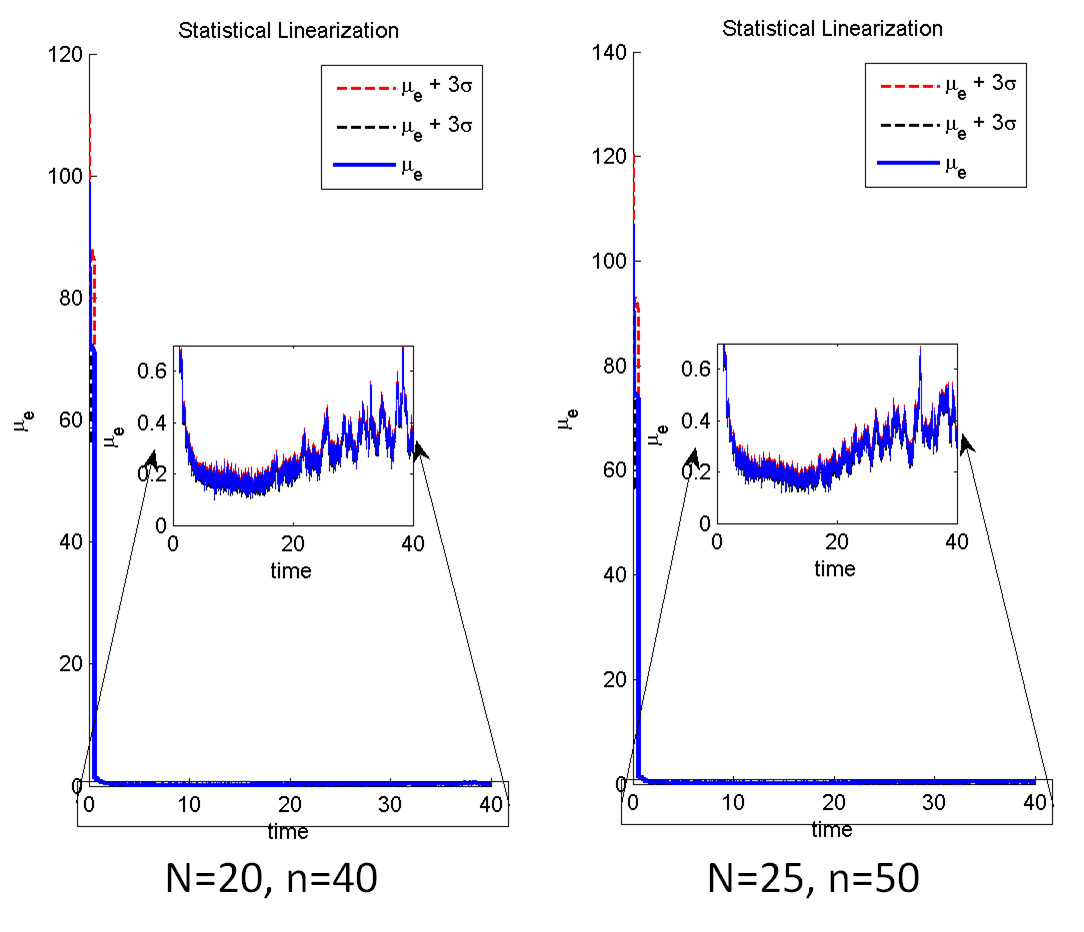
\includegraphics[width=0.8\textwidth]{figures/FIG_14}
\caption{Comparison of Original System propagation with that obtained from the two clustered model for Weakly coupled Van der Pol Oscillators after filtering}
\label{vanderpolhdcoup_clust_filter}
\end{center}
\end{figure}

From Figure~\ref{vanderpolhdcoup_clust_filter} it can be observed that the error in filtering is initially huge, and then the model approximates itself to the actual trajectory, and the error gets minimized. The average error in approximation given by $\bar{\mu}_e = \frac{1}{T}\mu_e$ has been tabulated. The time from start till the first observation is taking place is neglected for error computation. Table~\ref{vanderpolhdfilter} shows the tabulated error for some of the test cases. 

\begin{table}[H]
\scriptsize{
\begin{center}
\caption{Error in Filtering for Weakly Coupled Van der Pol Oscillators}
\label{vanderpolhdfilter}
\begin{tabular}{|c|c|}
\hline
$n$ & Statistical Linearization  \\ \hline
10    & 0.1002 \\ \hline
    20    & 0.1370 \\ \hline
    30    & 0.1998 \\ \hline
    40    & 0.2861 \\ \hline
    50    & 0.2994 \\ \hline
\end{tabular}
\end{center}
} 
\end{table}

\section{Summary}

The key contribution in the first work is the detailed study as to what extent a linearization and clustering algorithm is applicable to problem of UQ in weakly coupled dynamical system. The aim of this work is to find out the suitability of the application of the linearization and clustering algorithm to facilitate the technique of parallel computation. The usefulness of both \textit{time-domain} and \textit{space-domain} linearization has been shown through several numerical simulations on chaotic systems. With different combinations of dimension and coupling strength, the experiments are designed to increase the complexity of the test problem, posing a tough challenge for the linearization and clustering algorithm to detect the WCSs. The detailed analysis and the statistical test gives us an insight into the accuracy of the overall framework. The current method relies on linearizing the system at periodic time instances and hence the cluster structure is updated at regular intervals. Hence, such method can also be applicable to deterministic dynamical system, where the linearizing can take place with respect to the solution to the system of ODE at each time instance. It is to be noted that due to periodic updating of cluster, the identification of the cluster structure at each time instance is very important. Due to the chaotic nature of the test problems, wrong cluster structure identification at any time instance results in very high propagation of error for the future time. The ensemble of the subsystems provide an \textit{approximate} estimation instead of the \textit{exact} estimation for fast design and performance check. The test of hypothesis shows that the method of linearization and clustering works equally well, which also helps us to prove the claim of ergodicity made in Section~\ref{stat_lin_section}.

Going forward we have identified the Statistical Linearization as the preferred method of linearization due its ease in implementation and accuracy of approximation. The technique requires a one-time generation of realizations from the initial probability space. It is slower than Jacobian-based Linearization but proves to be faster and more effective than other time-domain techniques. 

The dependency of the method on the clustering technique gives scope of further research into incorporating new clustering methods into the framework. SC is easy to implement but computationally expensive for high dimensional systems. B-NMF is fast but the accuracy is often not guaranteed. The task of finding suitable clustering technique can be a never ending research given that new methods are developed every day. Furthermore, both the methods yield overlapping cluster information that can be normalized to obtain non-overlapping cluster structure. The question remains is how to efficiently utilize this overlapping cluster structure for the purpose of efficient UQ. This question is addressed in the next chapter.